\documentclass{tuftebook}

% Font and Encoding
\usepackage[T1]{fontenc}        % Font encoding
\usepackage[utf8]{inputenc}     % Input encoding
\usepackage{mlmodern}           % Latin Modern font

% Math and Symbols
\usepackage{amsmath}
\usepackage{amssymb}
\usepackage{amsfonts}
\usepackage{mathtools}
\usepackage{physics}            % For physics notation
\usepackage{amsthm}             % For theorems and proofs
\usepackage{cancel}             % For canceling terms in math

% Table and Formatting
\usepackage{booktabs}           % Better tables
\usepackage{caption}            % Customizing captions
\usepackage{float}              % Improved interface for floating objects
\usepackage{tabularx}           % Tables with flexible column widths
\usepackage{array}              % Extra functionality for tables
\usepackage{siunitx}            % For units and numerical data
\usepackage{arydshln}			% For Chapter 3

% Figures and Colors
\usepackage{pdfpages}
\usepackage{graphicx}           % For including graphics
\usepackage{xkcdcolors}         % XKCD colors
\usepackage{tikz}               % For creating graphics programmatically
\usepackage{tcolorbox}          % For colored boxes

% Algorithm and Listings
\usepackage{algorithm}
\usepackage[noend]{algpseudocode} % For algorithms
\usepackage{listings}           % For source code listings
\usepackage[table,xcdraw]{xcolor} % Color support for tables and code

% Hyperlinks and Metadata
\usepackage{hyperref}           % For hyperlinks
\hypersetup{
    colorlinks=true,            % Colored links
    linkcolor=blue,             % Color of internal links
    citecolor=blue,             % Color of citation links
    filecolor=magenta,          % Color of file links
    urlcolor=blue               % Color of URL links
}

% Additional Features
\usepackage{microtype}          % Microtypographical improvements
\usepackage{epigraph}           % For epigraphs
\usepackage{nicematrix}         % For nice matrices
\usepackage{empheq}             % Boxing equations
\usepackage{lipsum}             % Filler text

% Chapter Formatting
\usepackage[Sonny]{fncychap}    % Fancy chapter headings
\numberwithin{equation}{chapter} % Number equations within chapters
\frenchspacing                   % Use French spacing

\usepackage{theorem}

\begin{document}

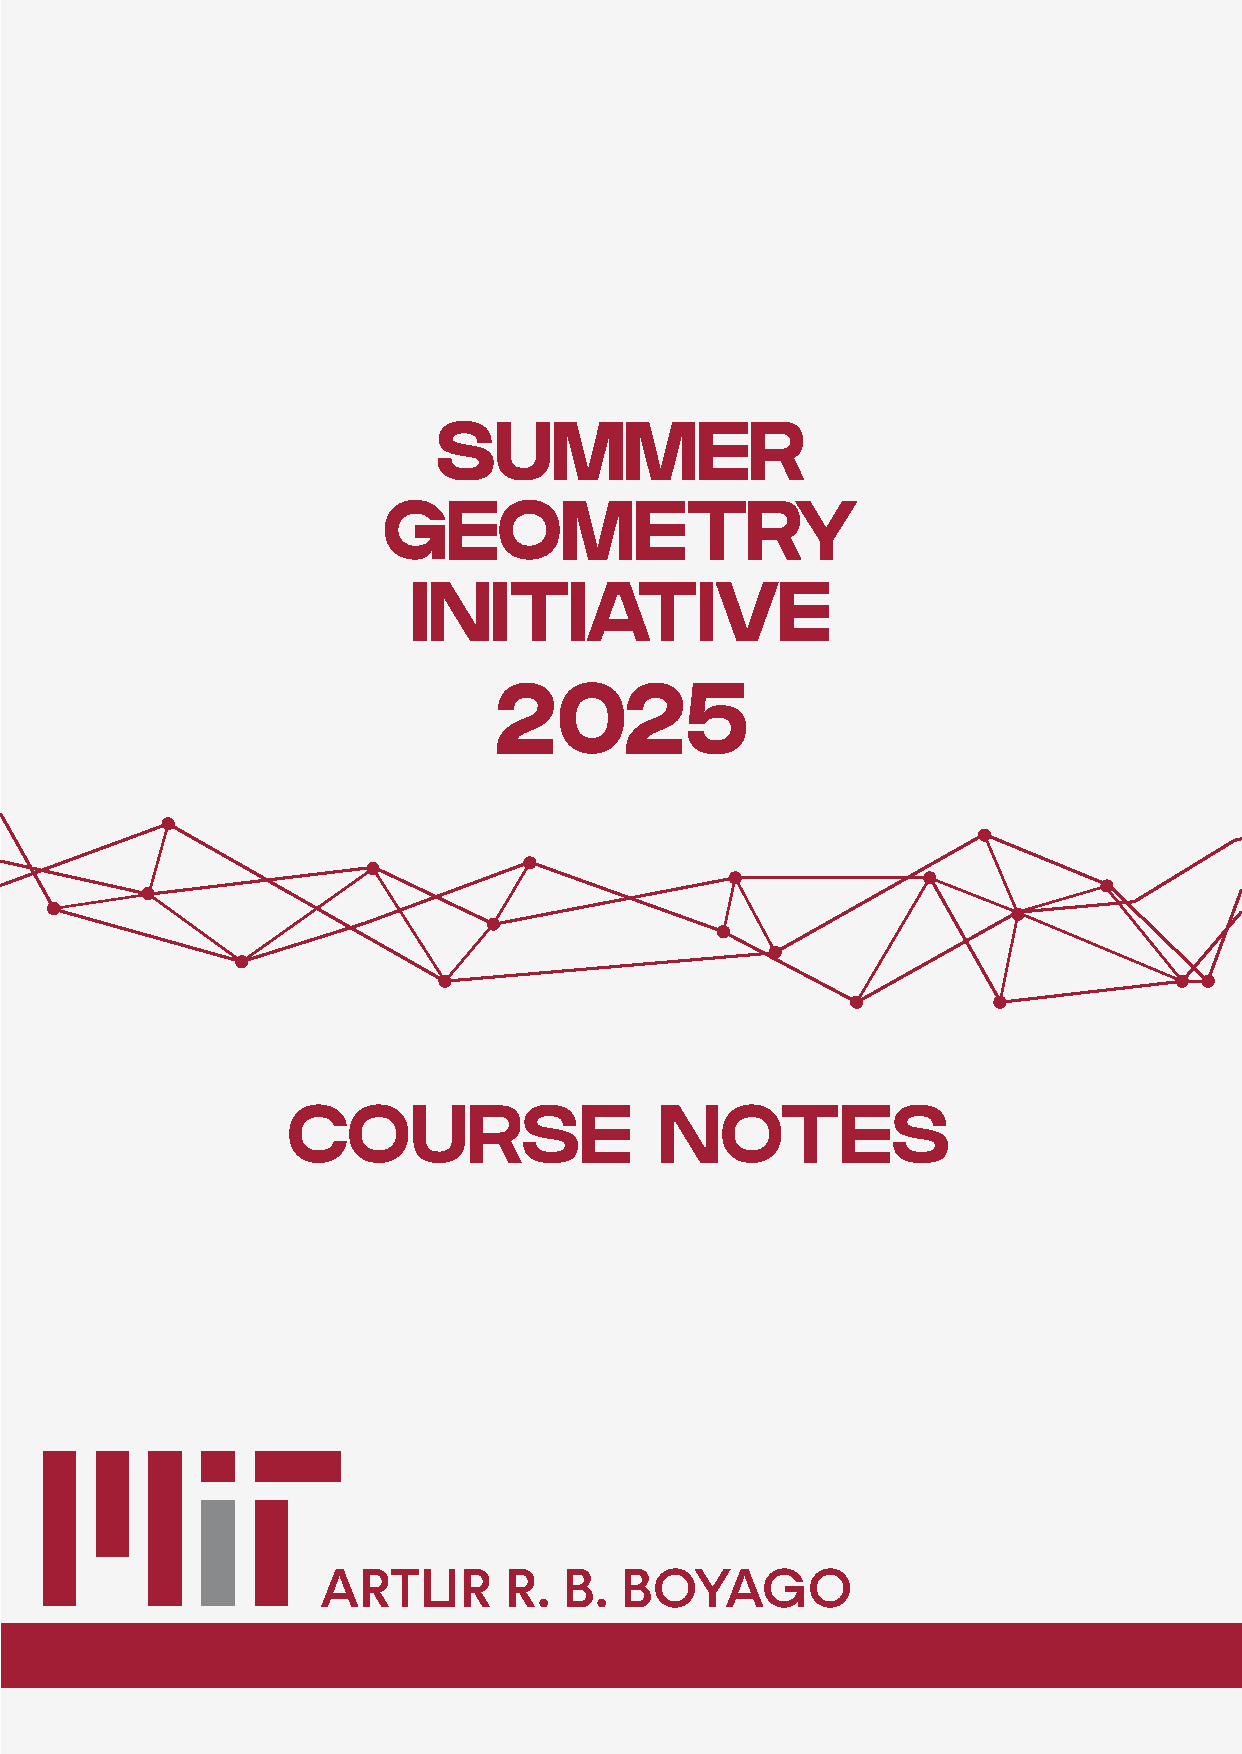
\includepdf[pages=1, fitpaper=true]{SGI_2025_cover.pdf}

\tableofcontents
\pagestyle{plain}
\chapter{Day 1}



\section{Mesh structure}

The general principle behind digital geometry processing is
approximating \emph{smooth manifolds} and the theory of
differential geometry regarding them to discrete scenarios.
We start by approximating manifolds and their properties.

\begin{marginfigure}
    \centering
    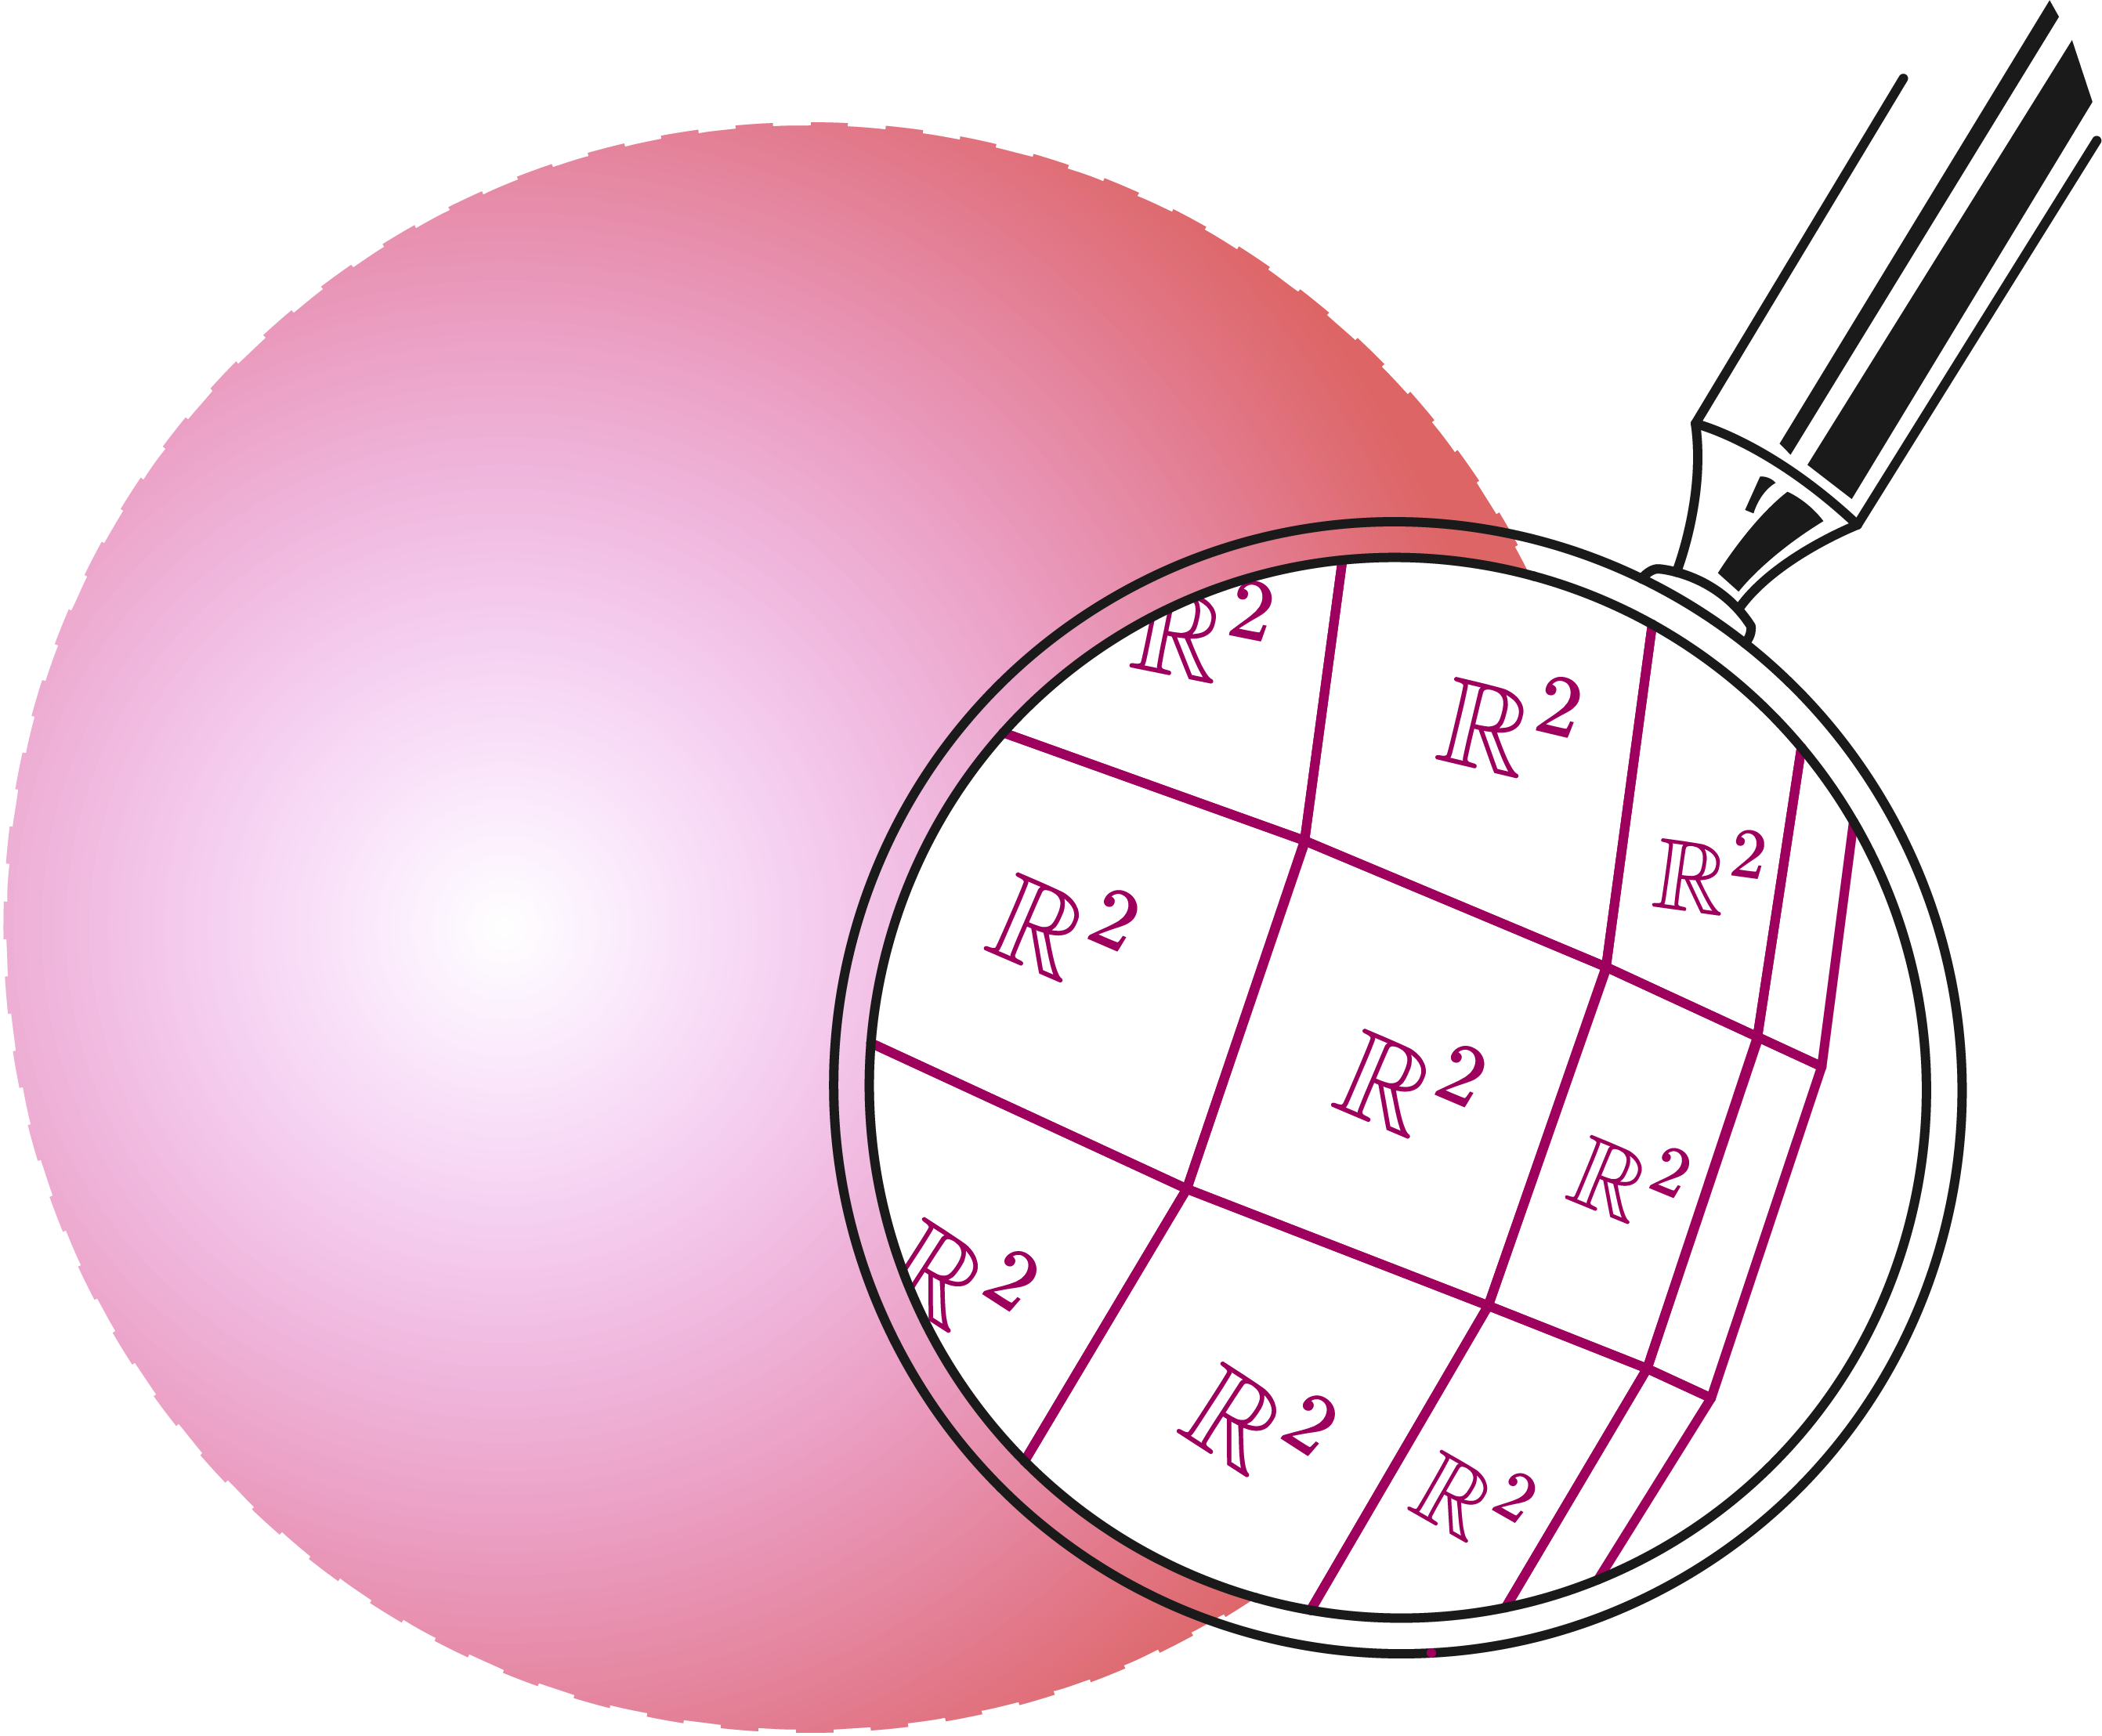
\includegraphics[width=0.8\linewidth]{images/sphere1.png}
    \caption{ A \textit{manifold} is a surface that under a microscope looks like
a flat sheet of paper, or $\RR^n$. Under the limit of 
infinite sheets of paper, you get a continous surface.}
\end{marginfigure}

\spa

A \textbf{\emph{mesh}} $\bf{M(V,E,F)}$ is a construction of some polygonal faces 
connected together, and the usual mesh is made up of rectangles or triangles 
stitched up together. You can make up the mesh by plotting the coordinates
of each of its vertices, at which point you get the
\emph{\textbf{vertex list}} $\Vsf \in  \RR^{n \times 3}$:

\begin{align*}
\begin{pmatrix}
\bf{v}^T_0\\
\bf{v}^T_1\\
\bf{v}^T_2 \\
\cdots
\end{pmatrix}
=
\begin{pmatrix}
x_0 &  y_0&  z_0\\
x_1 &  y_1&  z_1\\
x_2 &  y_2&  z_2 \\
&\cdots
\end{pmatrix}
=
\begin{pmatrix}
\text{1st Vertex}\\
\text{2nd Vertex}\\
\text{3rd Vertex}\\
\cdots
\end{pmatrix}
\end{align*}

Now, this gives us a nebulous little cloud of points. When you connect 
these little points together by some lines, you get \emph{edges} and a
\textit{\textbf{edge list}} $\bf{E}$;
get three of those in a loop, you get a \emph{face}. The faces of
the mesh compose a \emph{\textbf{face list}} $\bf{F}$. Therefore,
a mesh is composed of those three lists. \sidenote{One can also produce a
\textit{adjancency matrix} $\bf{A}$ \cite{benchen2010mesh} rather than
a edge connectivity list. This is related to how to inform directions in
planar graphs.}

\spa

In the same way as manifolds, lots of facts about algebraic and differential
topology can also be expressed for triangle meshes, namely 
topological invariants, which are numbers dependant only on the 
"qualitative characteristic" of the manifold at hand.
For example, per section 16.4.3 of \cite{realtime}, there is a very useful 
rule of thumb for roughly how many vertices, edges and faces a given triangular 
mesh will have, using the \emph{Euler-Poincaré formula} gives us
the \textit{Euler Characteristic} $\chi$:
\sidenote{A proof of this formula can be found in \cite{eulerpoincare1}}

\begin{definition}[Euler-Poincaré characteristic of a mesh]
    \begin{align*}
    \text{(Vertices) - (Edges)} + 2\text{(Faces) - (Loops)} + 2\text{(Genus)} = 2
\end{align*}
\end{definition}

\begin{marginfigure}
    \centering
    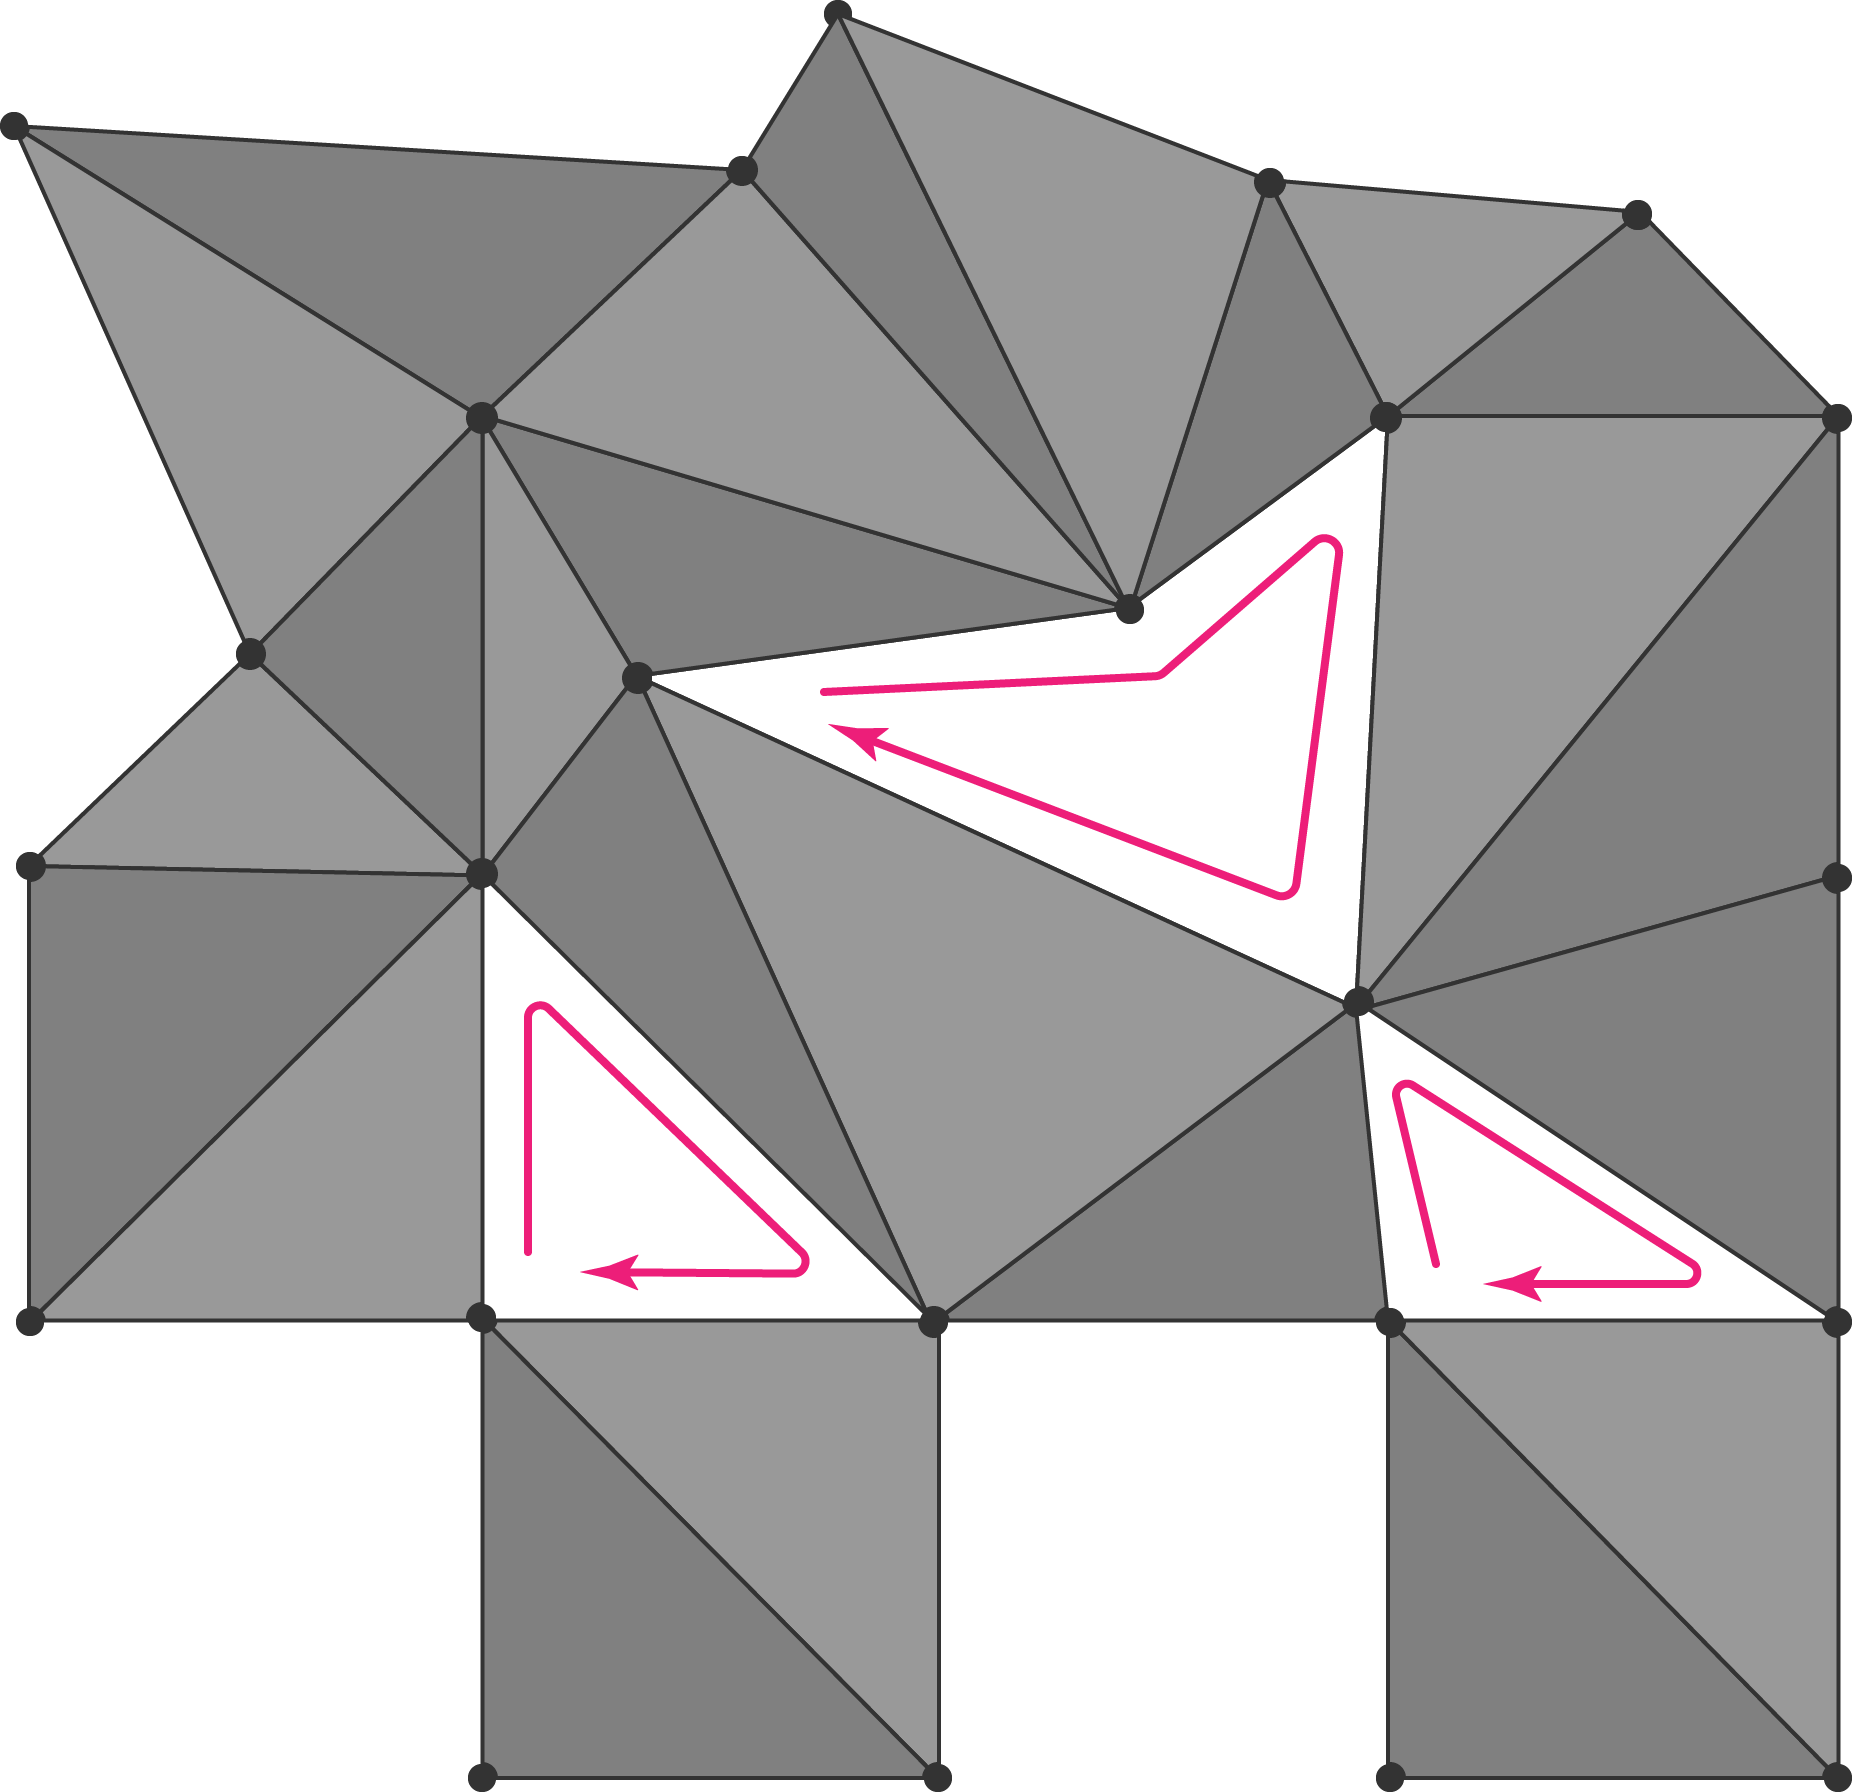
\includegraphics[width=0.9\linewidth]{images/meshloop1.png}
    \caption{An example grid mesh with 24 faces, 24 vertices,
    50 edges, three loops, a genus of 3. Indeed, one can see that
    applying these numbers into our formula gives exactly 2.}
\end{marginfigure}

The \textit{genus} would be "number of holes" in the mesh. It can be computed
by many means, for example, if we know the Euler characteristic of a mesh
as $\chi$, then $\chi = 2 - 2g$ \cite{weisstein_genus}.

For a closed (solid) model, every edge has two faces, and every face has at least
three edges, so $2e \ge 3f$. If the mesh is all triangles, as the GPU demands, then
$2e = 3f$. Assuming a genus of $0$ and substituting $1.5f$ for $e$ in the formula 
yields $f \le 2v-4$ If all faces are triangles, then $f = 2v-4$.

\begin{marginfigure}
    \centering
    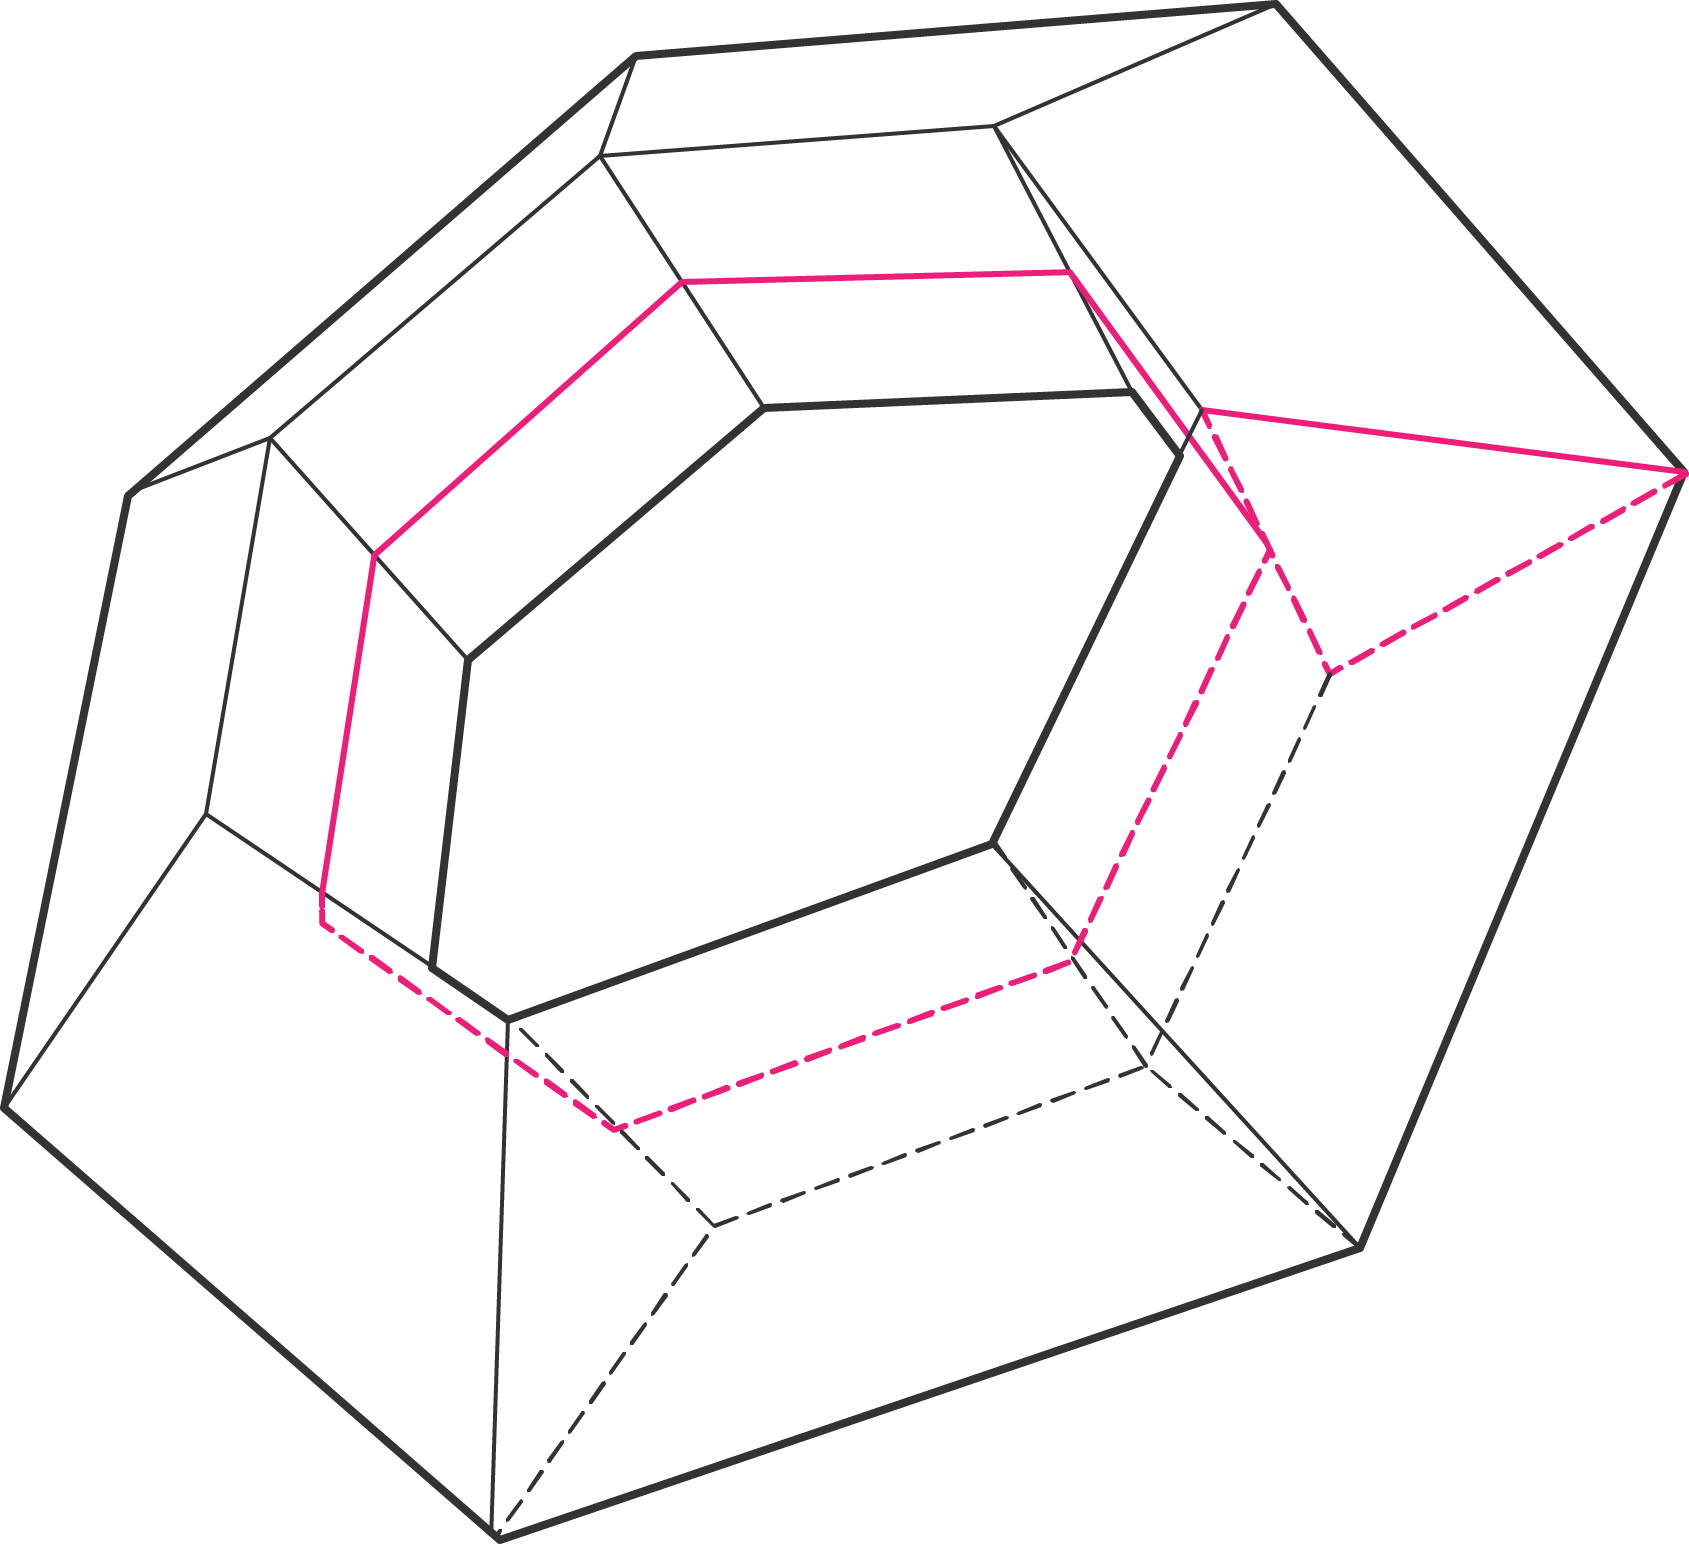
\includegraphics[width=0.8\linewidth]{images/donuttopology.png}
    \caption{A discrete torus mesh still contains many of the same topological
    properties of its continous counterparts. This can be understood in terms
    of an equivalence of graphs to the embedding diagrams of many of these figures.}
\end{marginfigure}

\section{Normals}

In 3D space, every little plane has a corresponding vector pointing
outwards out of it, orthogonally; the size of such a vector is proportional
to the size of the area of the little plane.

\begin{marginfigure}
    \centering
    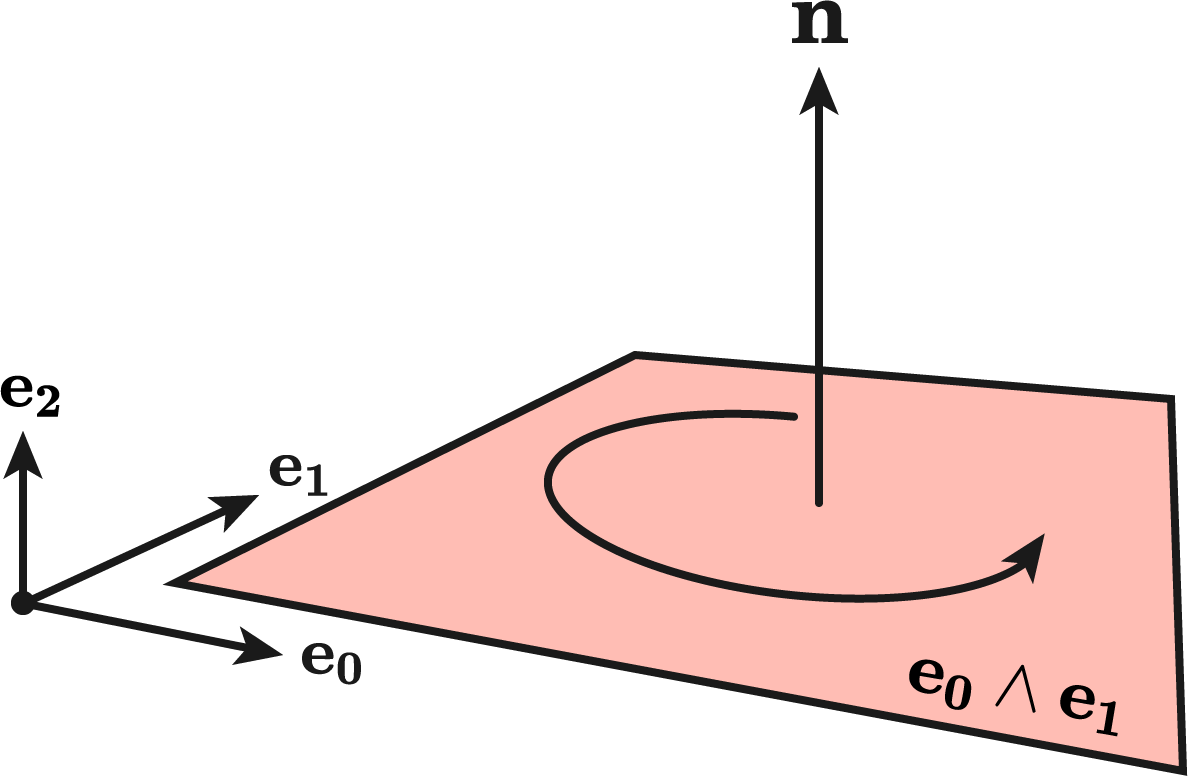
\includegraphics[width=0.7\linewidth]{images/bivectornormal.png}
    \caption{The plane represented by the bivector $\bf{B}$ generated
    by $\bf{e_0\wedge e_1}$ has a normal, axial vector 
    $\bf{n = e_0 \times e_1}$.}
\end{marginfigure}

\spa

You can make sense of this in many ways, but this is a property unique to
3D space. Using geometric algebra, one can very easily see two very
important properties that normals have, their \emph{orientation}
and the idea of \emph{normalization}. Indeed, if a mesh face or any general
plane is given by a bivector $\bf{B= a \wedge b}$, then the associated
\emph{\textbf{normal vector}} is the dual:

\begin{align*}
    \bf{n} &= \begin{pmatrix}
\text{Area of} \\
\text{plane}
\end{pmatrix}^{-1}
\begin{pmatrix}
\text{Dual of} \\
\text{said plane}
\end{pmatrix} \\
    &= |\bf{B}|^{-1} i\bf{B} \\
    &= |\bf{B}|^{-1} i(\bf{a \wedge b}) \\
\end{align*}

\spa

First, we see that normal vectors are \emph{pseudovectors} and not
real vectors. This is very important mathematically, as bivectors
(and therefore pseudovectors corresponding to said bivectors) behave
rather unusually under a given transformation matrix $\bf{M}$.
Whilst by basic linear algebra $\bf{v \rightarrow Mv}$, the
\emph{cross product}, or bivector, 
\href{https://peeterjoot.com/2024/01/21/bivector-transformation-and-reciprocal-frame-for-column-vectors-of-a-transformation/}{transforms}:

\begin{align*}
\bf{B} &\longrightarrow |\bf{M}| \bf{(B\wedge e_i) m^i} \\
 \bf{a \times b} &\longrightarrow (\text{adj } \bf{M})^T (\bf{a \times b})
\end{align*}

As pointed out in \cite{graphicscompendium},
if the surface was somehow deformed by some non-uniform scale transformation,
the rescaling matrix is not simply an inverse. This introduces all kinds
of extra complications when making algorithms for mesh deformations,
subdivision and etc, as one needs to be careful as to conserve the normals.

\subsection{Per-vertex normals / Pseudonormals} \label{per-vertex-normals}

A vertex is just a point, there is no inherent sense of direction
or magnitude associated to it; but it's convenient to want the normals
not associated to the faces, but the normals of a mesh. These are
also called \textit{pseudonormals} \cite{SDFnormal}.

\spa

So how does one do this? There are many somewhat equivalent
ways of choosing a normal. First, you have to choose a direction
relative to the vertex, and then a size. The basic idea is that
you can look at all the faces around you and their normals,
and take an average of all those normals:

\begin{definition}[Per-vertex normals]
    \begin{align*}
    (\text{Vertex normal}) = 
    \sum_{\text{Faces around vertex}} 
\begin{pmatrix}
\text{Normal vectors}\\
\text{from neighbour}\\
\text{faces to vertex}
\end{pmatrix}
\text{(Weight factor)}
\end{align*}

Which is written down normally (heh) as:

\begin{align*}
    \widetilde{\bf{n}_v} = 
    \sum_{f} \bf{n}_f w_f
\end{align*}

Where later on you just normalize the total normal
$\bf{n}_v$. 
The weight factor $w_f$ comes in three flavors of choice.
The last two are the most common:

\begin{itemize}
    \item \textbf{Uniform weighting:}
    We have that $w_f = 1$. The interpretation being that
    all face normals contribute equally to the total result.
    This "democratic principle" of vertex weighting is discussed
    below.
    
    \item \textbf{Area weighting:}
    We have that $w_f \propto A_f $, where $A_f$ is the area
    of the face. The larger the face, the more those normals
    contribute to the vertex normal.

    \item \textbf{Angle weighting:}
    We have that $w_f \propto \theta_f$, where $\theta_f$ is the
    angles subtended from the vertex to the other edges of the bounding
    faces. 
\end{itemize}
\end{definition}


\begin{marginfigure}
    \centering
    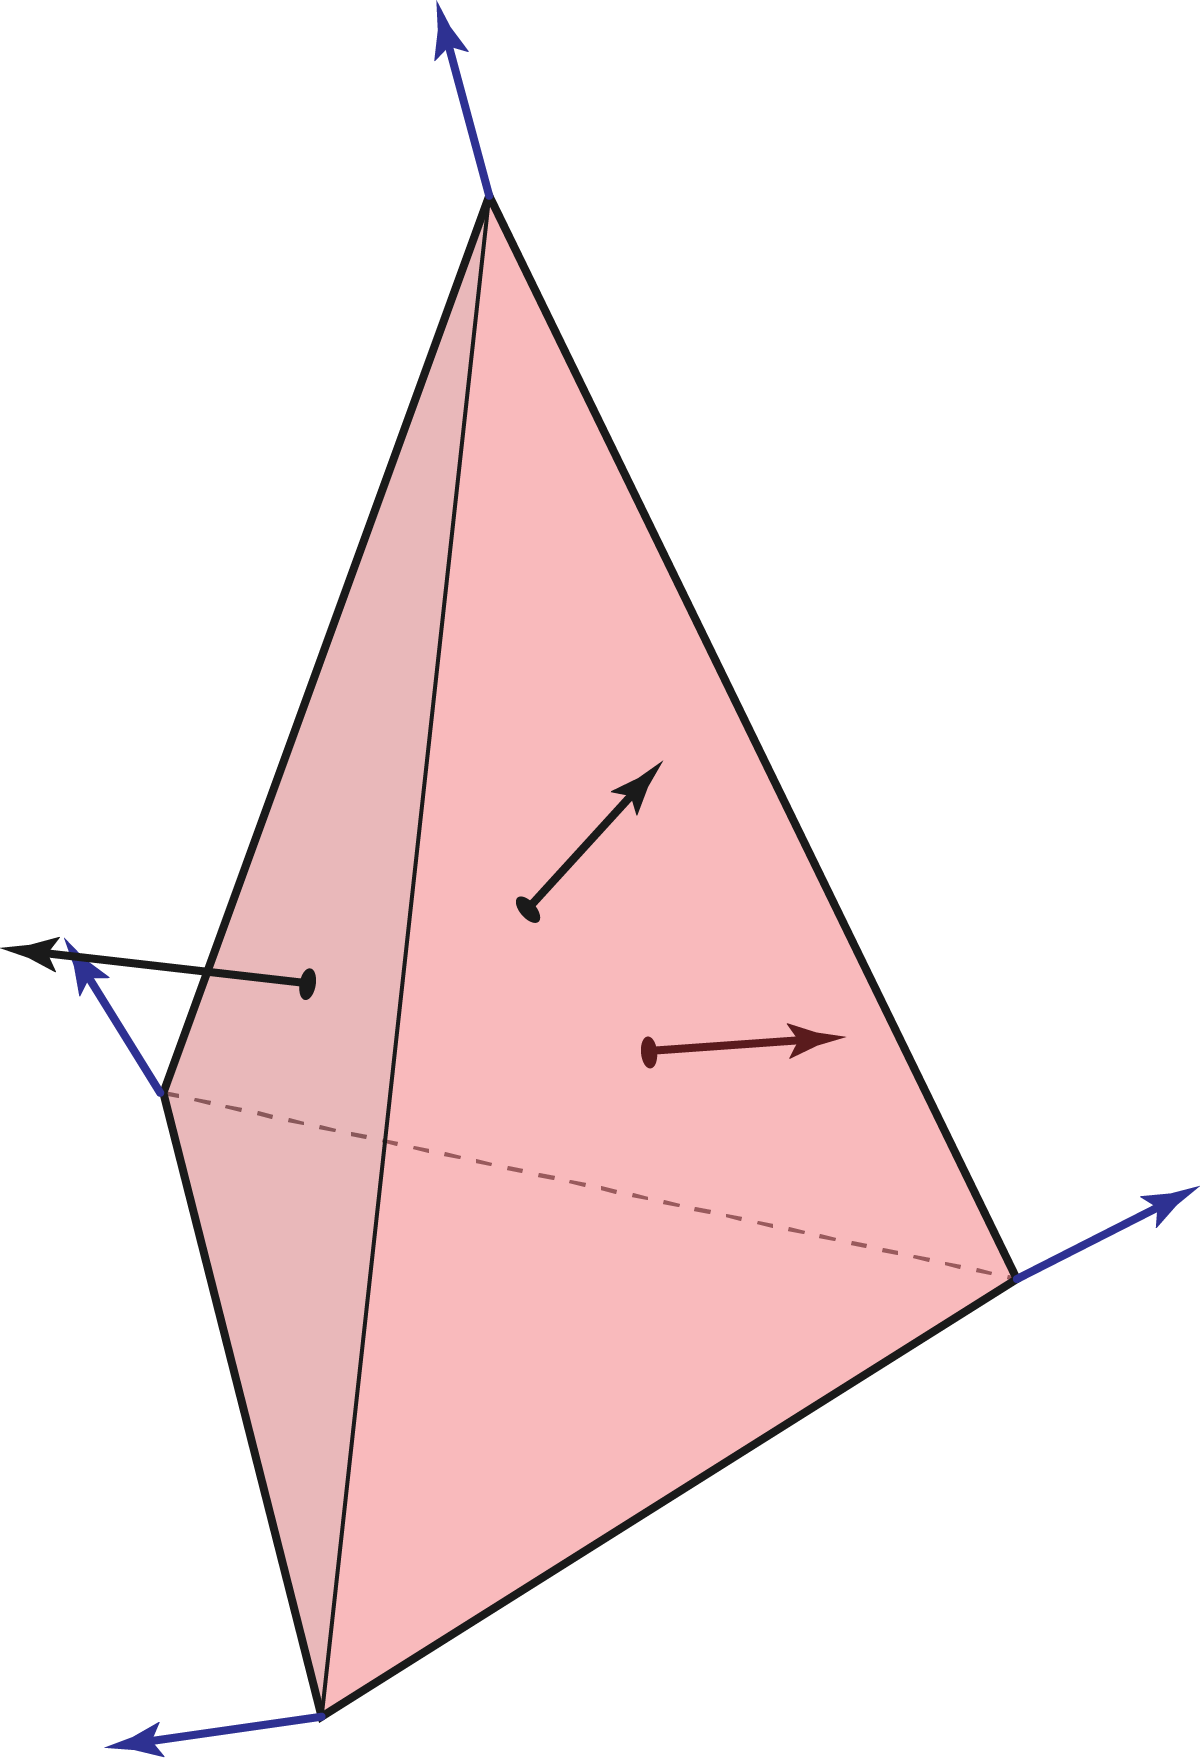
\includegraphics[width=0.8\linewidth]{images/pervertex.png}
    \caption{The face normals versus the area-weighted vertex normals
    of a simple tetrahedron without the bottom face.}
\end{marginfigure}

\spa

But why would we do these averaging procedures? Surely one can
just take all the normals around the vertex and average them
at once, like this:

\begin{align*}
    \bf{n}_v = \sum_i \bf{n}_f 
    (|\bf{n}_f|)^{-1}
\end{align*}

Not so \cite{vertex1}, one quickly
learns that if the faces around the vertex are sufficiently
distorted, even if the geometry remains the same, or that if one
adds \emph{more faces}, keeping the same geometry, one still gets
different vertex normals.

\spa

These three methods ensure that doesn't happen. The linked
paper claims the tesselation of the mesh doesn't affect the angle
method, so that would be generally better for geometric goals.

\spa

One can do a \textbf{shared normals scheme} as well, where
multiple normals can exist in the same vertex.
\section{Boundaries of Surfaces} \label{boundary}
%%https://en.wikipedia.org/wiki/Manifold#Manifold_with_boundary 


\section{Curvature} \label{curvature}

As discussed in \cite{discreteexterior1}, whilst curvature can be
easily defined in the continous setting, the discrete setting has no
trivial way of assigning curvature to surfaces due to the lack of 
differentiability and continuity in many functions. Therefore,
one can produce a \textit{array} of multiple discrete curvature
definitions, these that all approach the continous one at the
"infinite resolution" limit. For example, the basic curvature of a 
parametric curve $\gamma(s)$ is given by:

\begin{example}[Line gaussian curvature]
\begin{align*}
\kappa(s) = \frac{|| \gamma'(s) \wedge \gamma''(S) ||}{|| \gamma'(s) ||^3}
\end{align*}    
\end{example}


This scaled bivector area, a prelude to the generalized Riemann curvature,
\sidenote{The Riemman curvature is given as $\bf{Rie(a \wedge b)} = 
\partial_x \wedge \partial_y P_x(a) \cdot P_y(b)$ \cite{geometric_calculus1},
which is exactly a bivector to bivector function that maps the total
"area deficit" or "infinitesimal rotation generators" produced by local
spatial curvature. The deficit of the curve would exactly be the one
produced by its intrinsic curvature.}
gives us all the information we need, but in the discrete case, if
we're dealing with meshes and polylines, all vertex joints have
a "infinite" amount of curvature, and along the actual curve, none at all.
This can be remedied by doing a "cumulative check" over the whole arclength;
these curvature energy integrals then gives us a more \textit{global}
rather than strictly \textit{local} definition.

\begin{marginfigure}
    \centering
    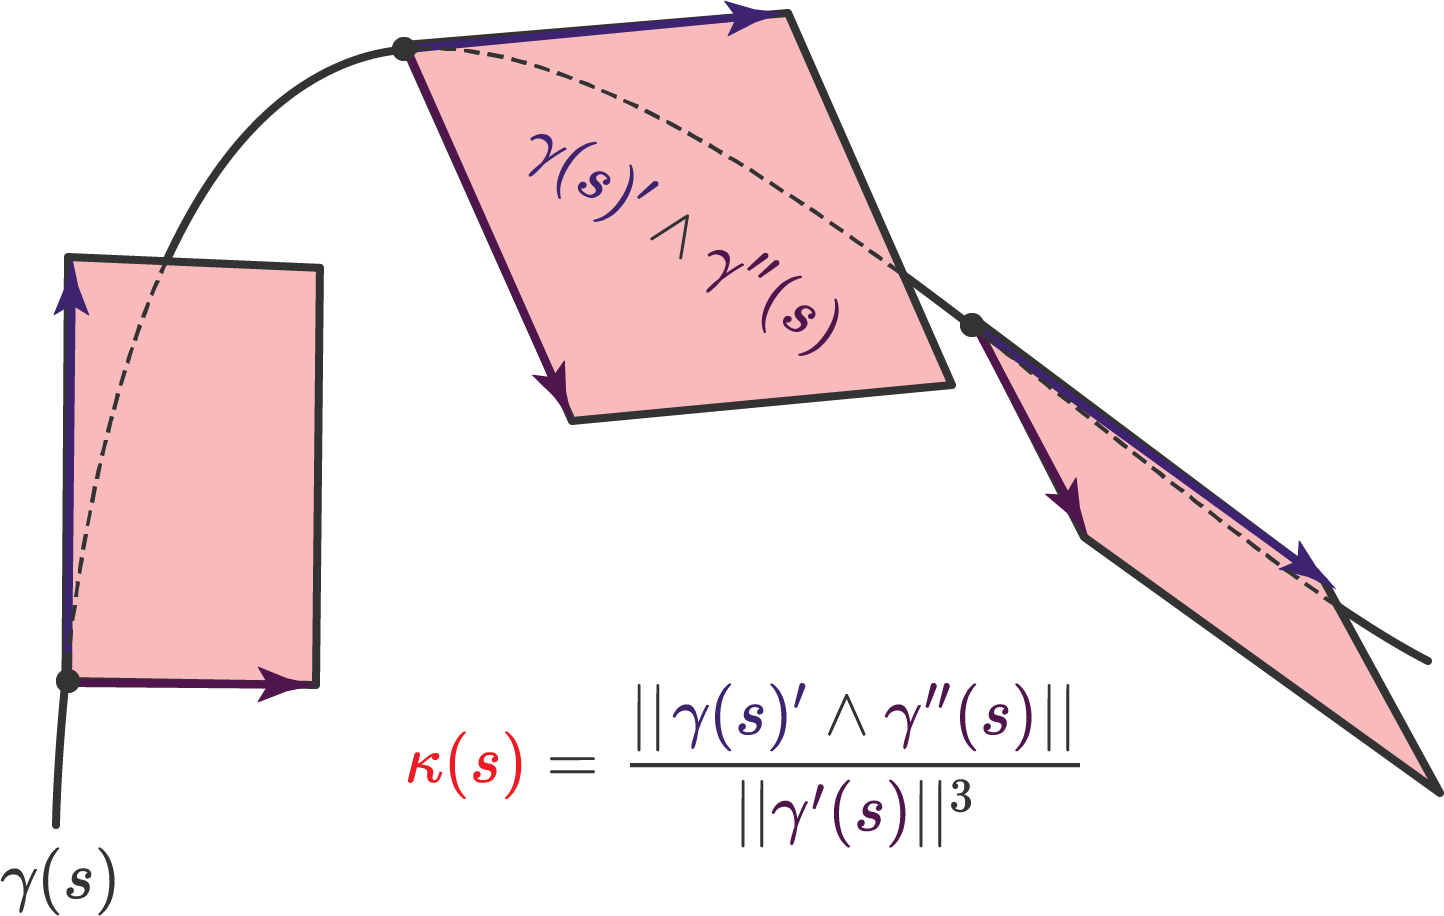
\includegraphics[width=1.0\linewidth]{images/curvature1.png}
    \caption{The curvature of a parametrized line $\gamma(s)$ is
    given by the reduced area of the bivector spanned by its velocity
    $(\gamma'(s))$ and acceleration $(\gamma''(s))$ vectors.}
\end{marginfigure}


\spa

We have four basic curvatures to deal with, \textit{\textbf{turning angle,
length variation, osculating circle}} and \textit{\textbf{Steiner's formula}},
all equivalent in the continous case, but inequivalent in the discrete one.
A complete description is in the \textit{discrete curvature 2} section of
\cite{discreteexterior1}.

\subsection{Turning angle}

The first curvature that was partially implemented in the course in
\ref{angle-defect-algorithm} was the \textit{turning angle} one, 
originally put in \cite{Crane:2010:TCD}, it approximates the associated
holonomy of edge loops along the entire mesh.

\spa

The idea is to compute two matrices, $\bf{A} = [d_0^T, \ H_{ij}^T]^T$
and $\bf{B} = [k, \ z]^T$, that give the number of contractible
and non-contractible basis cycles in a mesh, and the angle defects 
around said cycles corrected for the total Euler characteristic $\chi$
of the surface mesh.


\subsection{Riemann curvature and such}

In usual exterior calculus, the Riemann tensor is of the form
$F \approx d\bf{A} + \bf{[A,A]}$; the approximation using
discrete exterior calculus is to see variations in area/volume
in Delaunay triangulations. In \cite{exterior_calculus1},
the idea is that $\bf{Rie(a,b)}$ is:

\begin{align*}
R_v&=\frac{\sum_{h_{\mid v}} R_h A_h^* A_{h v}}{\sum_{h_{\mid v}} A_h^* A_{h v}} \\
 &=\frac{\sum_{h \mid v} R_h A_h^* A_{h v} / \sum_{h_{\mid v}} A_{h v}}{\sum_{h_{\mid v}} A_h^* A_{h v} / \sum_{h_{\mid v}} A_{h v}}
\end{align*}

\begin{align*}
\langle Q\rangle_v \equiv \frac{\sum_{h_{\mid v}} Q_h A_{h v}}{\sum_{h_{\mid v}} A_{h v}}
R_v=\frac{\left\langle R_h A_h^*\right\rangle_v}{\left\langle A_h^*\right\rangle_v}
\end{align*}

\subsection{Minimal surfaces}

A saddle is a good example of a minimal surface.
\cite{bouma2001}
\chapter{Day 2}

\section{Mesh Parametrization}

\begin{definition}[UV Maps]

The idea is we want to "squish" or "flatten" our 3D mesh into a snug
2D projection, an image. This produces a \emph{\textbf{UV map}}, and
the procedure in abstract is to assign a subset of 3D space 
$V$ contained by edges to a domain in 2D space $\Omega$:

\begin{align*}
    U: V\subset \RR^3 \rightarrow \Omega \subset \RR^2
\end{align*}
    
\end{definition}

If the edge is a closed object, like a cube, obviously if you try to squish
it, some bits of the cube will be on top of each other, so a no-go to
a UV map. What can be done is cheating; you cut some bits of the original
3D object first so that it becomes "flattable".

\spa

This procedure of incision is sucessful once we reach a
\emph{disk topology}, containing a single boundary loop. Some meshes
require that we make multiple seams and separate multiple sections into
little "UV islands"; this can be done for semantic or mathematical
purposes. Our objective in parametrization is to minimize
\emph{distortion} and the number of cuts.

\subsection{Springs algorithm (Tutte Embedding)}

A basic mesh parametrization algorithm treats the entire mesh as a
set of springs with different elastic coefficients; we want to
"relax" the whole mesh by allowing the springs to stretch until they're
flat and constrained to some boundary. This is known as a
\emph{\textbf{force-directing algorithm}} for making planar graphs.
A \href{https://www.youtube.com/watch?v=WWm-g2nLHds&list=PLubYOWSl9mIvtnRjCCHP3wqNETTHYjQex}{good playlist.}

\spa

This is the same as trying to minimize the potential energy $U$
of the entire system of springs.

\begin{align*}
\min_{U} \sum_{\{i,j\} \in \bf{E}} w_{ij}\bf{||u_j-u_i||}^2
\approx \min_{\text{Pot. energy}} \sum_{\text{vertices}} k\bf{x}^2
\end{align*}

We can numerically solve the relaxation of springs by looking at a basic
$2k\bf{x}=0$ idea:

\begin{align*}
\frac{\partial U}{\partial\bf{u}_i}=\sum_{\{i\,j\}} 2w_{ij} 
(\bf{u}_i-\bf{u}_j)=0 \approx 2k\bf{x}=0
\end{align*}

The spring potential $k$ represented by the stiffness of each edge
$w_{ij}$ can be adjusted to not be a constant, but rather depend on
something. Following \cite{param1stanford}, we have:

\begin{itemize}
    \item \textbf{Uniform weights:} The stiffness of every spring
    is equal. This relaxes them all into equilateral triangles.

    \item \textbf{Harmonic weights:} Dependant on adjacent angles
    between faces to imitate a conformal transformation. According
    to \emph{Lemma 1} in \cite{minimal1}, it comes about from
    minimizing the total discrete \emph{Dirichlet Energy}.

    \item \textbf{Mean-value weights:} Using barycentric coordinates,
    explained below, we can produce weights that are always positive
    and precise in the linear sense.
\end{itemize}

Following \cite{param2sheffer}

\spa

\subsection{Distortion}

The amount of distortion a mesh has is measured by the Jacobian, which
tells you the total infinitesimal variation in a volume element across
all directions.

\begin{align*}
    J_f = U\Sigma V^T = U
\begin{pmatrix}
\sigma_1 & 0\\
 0 & \sigma_2\\
 0 & 0
\end{pmatrix}
V^T
\end{align*}

We can split this into three cases.

\begin{itemize}
    \item \textbf{Area preserving (Equiareal):} 
    If $\text{det}(J_A^2)=\text{det}(J_B^2)$, this implies
    $\sigma_1 \sigma_2 = 1$.
    
    \item \textbf{Conformal (Equiangular):} If there exists a scalar function
    $\phi(u,v)$ that perfectly offsets the variation of the original
    area, such that $J_A^2 = \phi J_B^2$, this is conformal, and it
    implies $\sigma_1=\sigma_2$.
    
    \item \textbf{Isometric:} If the transformation is both
    conformal and equiareal, then it is isometric, and therefore implies
    $J^2_A = J^2_B$, which implies $\sigma_1=\sigma_2=1$.
\end{itemize}

\href{https://github.com/alecjacobson/geometry-processing-parameterization}{Jaconson's course}

\subsection{Barycentric Interpolation}

As per the original floater article \cite{floater1}, as well
as his more explanatory article \cite{floater2}, the basic idea is that
the coordinates \emph{inside} of a triangle $T$ composed of vertices
$\bf{v_1, v_2}$ and $\bf{v_3}$ are linear superpositions of the
vertices scaled by a ratio of the area of the triangles formed by each
vertex and the total triangle area:


\begin{align*}
\bf{x} &= \lambda_1 \bf{v_1} + \lambda_2 \bf{v_2} 
+ \lambda_3 \bf{v_3} \\
\\
\lambda_i&=
\begin{pmatrix}
\text{Area of} \\
\text{triangle made of} \\
\text{base edge } \bf{v}_i
\end{pmatrix}
\bigg/
\begin{pmatrix}
\text{Total area} \\
\text{of triangle}
\end{pmatrix}
\end{align*}

The construction can actually be generalized to any convex polygon
(altough not at all polygons will produce bijective maps \cite{barycentric1})
but we'll stick to triangles. The original motivation of this
system was to mimic \emph{harmonic maps} by piecewise linear maps, that
is, allow a conformal transformation to be more easily carried out.

\spa

Suppose we had a harmonic function $\Delta f = 0$. If we wish to
approximate $f$ by regarding a boundary condition 
$u(\partial \Omega) = u_0$. We want to produce some triangulation
$\mathcal{T}$ whose values of interior edge lengths and angles
look like a conformal map. This then produces a system of equations
that is exactly that of mean value, or barycentric coordinates.

\spa

For mesh parametrization, we want to follow
the procedure outlined in section 5.4 of \cite{floater2}.
Suppose we have a mesh $\bf{M}(E,V, F)$, where $E$ are its edges,
$V$ its vertices and $F$ its faces. Then the \emph{boundary of the mesh}
$\partial\bf{M}$ produces a \emph{boundary polygon}.

\spa

Our goal is to, as per the Tutte embedding, map the boundary polygon
into another convex polygon fixed in the UV plane, and then make all
other triangles of the mesh be convex combinations of their neighbors
in such a fashion as to fill the UV plane.

\spa

Mean coordinates can also be extended to non-convex polygons.

\section{Texture mapping and optimization}

\subsection{Mapping}

Supposing we express a mesh $\bf{M(u,v)}$ in these UV coordinates,
we can store image data in the UV plane and then map this back to the
original mesh to get colors on our mesh.

\spa

The basic method is a \emph{\textbf{triangle soup}} mapping, which
obliterates connectivity information in return for a completely
isometric mapping to the UV space.

\subsection{Optimization}

\section{Level of Detail (\emph{Nicole Feng})}

There's a great deal of difficulty in rendering models
with a lot of details, due to the computational cost.
This originally motivated artists to produce 
different versions of the same object in different
levels of detail, that is, number of polygons,
quality of textures, to save the performance.

There are several issues with this however. The 
first of course is the sheer volume of work; in
some video games, we have thousands of assets. 
We'd have to manually produce three or four versions
of each asset if we'd like to generate accurate LODs
for each one, which is unfeasible.

Further, one can have many transition artifacts
between the low and high LOD versions of the same
object, known as \emph{pop-in}. beyond
straightforward videogames, any kind of
application that consumes large amount of memory
require LOD systems for efficient computing,
in MRI for example.

It would be of our interest to somehow make this
process automatic and very much seamless.

\begin{itemize}
    - What does detail mean?

\end{itemize}

Taylor expansions and fast multipole methods
can be seen as LODs.

\subsection{1D curves}

Let's suppose we have a polyline
$\gamma(t)$ given by some sequence of points
$S$, which contains the vertex positions 
and the connectivity information.

Let's produce a low detail version of the
polyline. Intuitively, we could remove one 
of the vertices or the edges in some kind 
of choice heuristics in order to make it
have less points whilst preserving its 
geometry. We then need some metric to 
tell us \emph{what} exactly is
a similar curve, an error metric.


Minimizing squared distance

A fairly simple error metric is to determine
the average squared distance from the original
polyline.



We retain information from the original
curve, as reference to further iterations.

\subsubsection{A smooth to discrete example of LOD}

Suppose we had a curve $A(t):[0,1] \rightarrow \RR^n$,
and we want to build an \emph{approximate} polyline curve
$B(t)$. We want to make our discrete points have the nearest
look to our original curve $A(t)$. 

\spa

As such, we must choose an \emph{error metric} measuring how
similar the two curves are, and make an algorithm that produces a
curve that minimizes this metric. A basic one is simply to measure
the total \emph{area} separating the approximate and real curve,
and attempt to minimize it.

\begin{figure}[h]
    \centering
    \includegraphics[width=0.7\linewidth]{images/error1.png}
    \caption{Basic error metric}
\end{figure}

\spa

The \emph{distance} between the polyline and the curve is
defined as the \emph{Chamfer Distance} \cite{chamfer1}
of the two sets of points $ch(A,B)$. One can also use the analogous
\emph{Hausdorff Distance} \cite{chamfer3}; ultimately, both
look at the the minimizing or maximizing, respectively, distances between
the two sets. Along the curve integral one can imagine the Hausdorff
metric produces a \emph{mean} value for the error, whilst the Chamfer
metric produces an absolute amount.

\begin{figure}[h]
    \centering
    \includegraphics[width=0.75\linewidth]{images/chamfer1.png}
    \caption{Chamfer distance produces,
    among evenly sampled points, circles.
    The nearest points are the radius of
    said circles that touch the curve $A(t)$.}
\end{figure}

Where the element $d(A,B)$ is indeed the Euclidean distance.
It makes sense then that the associated integral
becomes a running integral over the Chamfer distance
of the two curves:

\begin{align*}
    \text{(Total error)} = \int_{[0,1]} ch(A,B) 
\end{align*}

And we'd like to readjust and resample $B(t)$ to
minimize this cost functional. Let us discuss, besides Chamfer, some 
other useful error metrics.

\subsection{Different error distances}

Let $X$ be a compact, smooth submanifold in $\RR^3$ 
that inherits the Euclidean metric from $\R^3$, i.e., a closed
surface (like a sphere or a torus) or surface with boundary (like 
a purse). We consider two measures of the \emph{dissimilarity} between 
two sets and their numerical proxies, and apply these two 
measures for $X$ and its deformed mesh $f(M)$ in particular. The 
two measures of dissimilarity are given below.


\begin{figure}
    \centering
    \includegraphics[width=0.8\linewidth]{images/frechet1.png}
    \caption{The Fréchet Distance is nothing but the distance between
    points that have the same parametrization.}
\end{figure}

\begin{figure}[h]
    \centering
    \includegraphics[width=0.8\linewidth]{images/frechet2.png}
    \caption{The \emph{free-space diagram} associated to a 
    8-unit distance contour around the curves and the respective
    red intersection.}
\end{figure}

\begin{figure}[h]
    \centering
    \includegraphics[width=0.8\linewidth]{images/frechet3.png}
    \caption{Two intersecting squiggly curves.}
    \label{fig:enter-label}
\end{figure}


\begin{figure}[h]
    \centering
    \includegraphics[width=0.8\linewidth]{images/frechet4.png}
    \caption{Evaluation of "nearest-point" Chamfer distance along the
    two squiggly curves.}
\end{figure}


\begin{figure}[h]
    \centering
    \includegraphics[width=0.8\linewidth]{images/frechet5.png}
    \caption{Proper, parametrized Frenet distance between curves, now
    showcasing that since the parameters are all mismatched, one can get
    shape information.}
\end{figure}


\subsection{Polyline algorithm}

Once again, we have a curve $A(t)$ that we'd like to approximate
by a polyline $B(t)$; we'll have data composed entirely of simply connected
points in the matrix $\bf{V}$ with some "direction information" 
stored in the order $\bf{v_i\rightarrow v_{i+1}}$ of rows.

\spa

If our space is $n-$dimensional we'd have $n$ columns to 
$\bf{V}$, for now we'll only worry about 3, so we have a
$\bf{V}$ of size $(k \times 3)$, where $k$ is the number of
vertices for $B(t)$.



\subsection{2D surface examples}

We once again have a triplet $(\mathbf{M,E,V})$
containing the vertex positions and connectivity
information. We can extend the same quadric
error metric approach to the surface.


\subsection{Mapping between levels}

\emph{Continous LOD} generates a data structure 
to interpolate between different LODs in such a way
that it looks seamless. 

\begin{align}
    \sum \mathcal{O}
\end{align}

Whenever we do a simplification to a mesh
containing a texture, we need to update the
colors in a way that doesn't distort the colors.

\subsubsection{Multigrid/resolution methods}



\chapter{Day 3}

\section{Geometric data}

It takes much effort to represent shapes in a virtual environment. Since
we only have finite memory and processing power, it is wise to implement
different data types for representing different constructs.

\spa

For example, when scanning real objects we're not really able to infer the
contextual information regarding certain features; therefore, we end up with
simple points in 3D space, which are clouds, but if you want to represent something
akin to a curve or do precision engineering work, you might want a mathematically
parametrized surface, since those don't suffer from finite resolution and can
be modified indefinitely.

\begin{table*}[h] \centering
%\ra{1.3}
\begin{small}
\begin{tabular}{@{}lll@{}}\toprule
\textbf{Data Type} & \textbf{Dimen.} & \textbf{Note} \\ \midrule
\textbf{Point clouds} & 0/3 & 52  \\ \hdashline
\textbf{Polylines} & 1/3 & 88  \\ \hdashline
\textbf{Splines} & 1/3 & 71  \\ \hdashline
\textbf{Implicit Surfaces} & 2/3 & 60  \\ \hdashline
\textbf{Parametric surfaces} & 2/3 & 55\\ \hdashline
\bottomrule
\end{tabular}
\end{small}
\caption{Data types and their corresponding co-dimensionality as well
as use in embedded spaces. Point clouds are, for example, 0-dimensional
entities that can be embedded in 3D space.}
\end{table*}

\subsection{Point Clouds}

Still don't know much about them besides just being an aggregate cluster of
coordinates.

\subsection{Splines / Curves}

Discretize a curve $\gamma(t)$ into a set of finite points
by using splines, which are simple parametrizations that obey
certain differentiability rules; see 
\href{https://www.youtube.com/watch?v=aVwxzDHniEw}{Freya Holmer's talk
on Bezier's} and on the 
\href{https://www.youtube.com/watch?v=jvPPXbo87ds}{the continuity of
splines}.

\subsection{Implicit Shape Representations}

\emph{Implicit Shape Representations} are of the form 
$f(\bf{x})=0$; this differs from \emph{parametric} forms
of characterizing $g(u,v)$. One of the major advantages is the
ease of computing intersections \cite{ray1} by means of a
bounding hierarchy and a simple algorithm to check
wheter a ray $\bf{r}(t)=\bf{a}+t\bf{b}$ crosses
it or not.

\spa

Further, these implicit surfaces can also have constructive
geometric operations applied to them very easily. An example is
a basic \texttt{AND/OR} algorithm by taking the $\min$ and
$\max$ of the two functions, or the deformation of
\emph{meta balls}, which is a set of sum of gaussians.

\subsection{Signed Distance Functions} \label{SDFs}

Following \cite{wave1} and \cite{SDF1}, a \emph{SDF} is a function that
determines the \emph{distance} from an arbitrary point in space to the
object in question. In 2D space, for example, imagine we had
a shape $\mathcal{S}$, and we pick some arbitrary point 
$\bf{x}$ in the space around the shape, $\mathcal{M}$. We want
a point $\bf{p} \in \mathcal{S}$ that \emph{minimizes} the distance
function between the point in the shape and the point in space:

\begin{align*}
    \min \text{distance}(\bf{x}, \cal{S}) = d(\bf{x,p})
\end{align*}

To produce the function 
$\text{SDF}(\bf{x,p}) : \RR^n\rightarrow\RR$ that
takes a point in $n-$dimensional space and spits out a distance scalar,
we add an aditonal constraint to this distance function:

\begin{align*}
\text{SDF}(\bf{x,p}) =
\begin{cases}
\ \ d(\bf{x,p}), \quad \text{if }\bf{x} \notin \mathcal{S} \ \text{(exterior)}
 \\
-d(\bf{x,p}), \quad \text{if }\bf{x} \in \mathcal{S} \ \text{(interior)}
\end{cases}
\end{align*}

That is, if you pick a point \emph{inside} the shape, it'll also
register the distance, but it'll be negative. The points \emph{on}
the shape have 0 distance, and so are not signed. There are also
simpler but less used \emph{indicator functions} that return 1 outside
and $-1$ inside.

\spa

One can have \emph{exact} and \emph{approximate} SDFs. An 
\emph{exact} SDF obeys the \emph{eikonal equation} $|\grad f| = 1$, as is
explained by \cite{wave1} in equation 6. The idea being very simple:
imagine we have a tank of water, and we twist a metal wire in the shape 
we want, and then we \emph{splash} that shape in the water.

\spa

The outward and inward propagating waves out of this splash produce
exactly the level sets of distance of our shape; so, if we compute how
a wave propagates in that way, and grab the level sets or the wave fronts
of the wave over time, we get the SDF. We can also prove the eikonal
condition using some functional inequalities \cite{wave2}.

\spa

Now to render and use these things we want to do some kind of algorithm
that checks the closest point to the shape at any moment. This is pretty
trivial to do with \emph{sphere tracing}. As the name implies, you pick
some point $\bf{x}$, draw a \emph{circle} $C$ around said point,
and start expanding its radius. At some point it'll touch some bit of
the shape, and that's the nearest bit to $\bf{x}$ \cite{SDF2}.
Easy right?

\spa

To construct more sophisticated SDFs we wish to use methods
to join basic, exact SDFs into other, more complicated shapes.
The basic procedure is to apply various \emph{boolean operations}
to the SDF, union, intersections and such, that produce new SDFs.
I'm not sure how this procedure is exactly done yet.

\subsection{Conversions between geometric representations}

Some things are impossible to do in certain representations. Animations
are near-inconceivable using parametric surfaces, but trivial in meshes.
How does one convert between these types of objects, without losing too
much information?

\chapter{Day 4}

\section{Mesh Simplification and Level of Detail}

Meshes contain a lot of geometric information for rendering processes,
and depending on the distance or size of said mesh, it's impractical to keep
the same number of vertices of a mesh in a close-up state and a far-away state.
This is solved by a \emph{LOD} system that transitions from larger to lower
number of polygons the further away or the less visible a mesh is.

\spa

Similarly, in the 1980s for example, methods that produced medical imaging
generated meshes with thousands of polygons, obviously overloading the
processing power at the time; it is then of our interest to somehow diminish
the amount of memory and processing required by lowering the number of triangles,
whilst keeping the shape and general details the same. So we have three major
types of mesh simplification \cite{realtime}:

\begin{itemize}
    \item \textbf{Static:} Static simplification is the idea of 
    creating separate level of detail (LOD) models before rendering begins, 
    and the renderer chooses among these.
    
    \item \textbf{Dynamic:} Gives a continuous spectrum of
    LOD models instead of a few discrete models, and so such methods 
    are referred to as continuous level of detail (CLOD) algorithms
    
    \item \textbf{View-dependant:} Where the level of
    detail varies within the model.
\end{itemize}

\spa

Two major methods were introduced to solve this at the time:
\textbf{\emph{global}} and\textbf{\emph{local}} methods for
LOD. The global method was explored by \cite{Hoppe1} and \cite{turk1}, 
whilst local methods were mostly developed by \cite{schroeder1}. 
However, many methods have been further debveloped over the years, and
many error metrics associated to the production of the coarser meshes
have arisen.

\spa

For example, rather than seeing how crooked the coarse mesh is
by some geometric argument, you can use the total screen-space
deviation of the original compared to the new mesh, as we would
only care about what we see in our screens.

\section{Dynamic simplification and Quadric Error Metric}

Developed by \emph{Pixar} in \cite{LOD1}, the idea is to produce a
sucessive series of \emph{edge collapses} to reduce the total number
of vertices and create a simpler model. The edge collapse procedure
takes two vertices $\bf{(v_1,v_2)}$ and maps them both to a new
vertex $\bf{v_3}$. This is usually written 
$\bf{(v_1,v_2)} \xrightarrow{\text{collapse}} \bf{v_3}$, and
removes one vertex, three edges and two faces.

\spa

The first question is where to put this new vertex $\bf{v}$; the answer
was to produce a cost function $Q$ based on the signed distance from the nearest
points of the vertex and the plane: a \emph{quadric error} is the smallest squared distance from a point to planes, so we have:

\begin{align*}
    Q &= \sum_i \ (\bf{n}_i \cdot \bf{v} + d_i )^2 \\
    &= \sum_i 
\left [ \begin{pmatrix}
\text{Plane} \\
\text{normal}
\end{pmatrix}
\cdot
\begin{pmatrix}
\text{New vertex} \\
\text{position}
\end{pmatrix} +
\begin{pmatrix}
\text{Plane offset} \\
\text{from origin}
\end{pmatrix} \right ]^2
\end{align*}

And we want to minimize this $Q$ to find $\bf{v}$.
Derek Liu's explanation of this went like this; first we
express this $Q$ in terms of matrices such that we implement it
in a linear solver. Ignore the $d_i$ correction term, and express
$\bf{v}$ as $\bf{(x-p)}$, where $\bf{p}$ is in the plane
and $\bf{x}$ is outside it:

\begin{align*}
    Q(\bf{x}) &= (\bf{x-p\cdot n})^2 \\
    &= \left \langle \bf{(x-p)n} \right \rangle^2 \\
    &=\left \langle \bf{(xn-pn)} \right \rangle^2 \\
    &=\left \langle \bf{(x\cdot n-p\cdot n)} \right \rangle^2 \\
    &=\bf{(xn)^2- 2(x\cdot n)(p\cdot n) + (pn)^2}
\end{align*}

Now we transfer from geometric algebra to matrix notation:

\begin{align*}
    Q(\bf{x}) &= \bf{(n^Tx)^2- 2(n^Tx)(n^Tp) + (n^Tp)^2} \\
&= \bf{(n^Tx)^T(n^Tx)- 2(n^Tx)(n^Tp) + (n^Tp)^T(n^Tp)} \\
&= \bf{(x^Tnn^Tx)- 2(nn^Tp)x + p^Tnn^Tp} 
\end{align*}

We can then simplify $\bf{nn^T = A, (nn^Tp)^T = b}$ and
$\bf{p^Tnn^Tp = c}$. This produces a quadratic equation
$Q(\bf{x}) = \bf{x^Tax + 2b^Tx + c}$. To \emph{minimize}
this function we only take the derivative and equal it to zero,
yielding a single linear solve for us to handle. When solved,
this gives us the $\bf{x}$, or in the original cost,
$\bf{v}$, that gives us the new simplified edge.

\spa

According to section 5.1 of \cite{LOD1}, the matrix $\bf{Q}$
used for finding optimal vertex positions will be invertible as long as the
level surfaces of the \emph{quadrics} generated by the quadratic equation
in plane space, are non-degenerate ellipsoids. In this case,
$\bf{v}$, our desired vertex, will be at the center of the ellipsoid.

\spa

There is a fairly intuitive interpretation \cite{LOD2}; the inner product will measure the cost
based on the "normal like" projected component of $\bf{x}$ onto $\bf{n}$;
within a concentric circle centered around the axis of $\bf{n}$, all $\bf{x}$
have the same projection. Changing the projection value produces an ellipsoid for all
collections of concentric circles. Indeed the surface of constant values of $Q$
measures the set of all points with a fixed error.

\section{Other Quadric Error Metrics}

There are many other of these quadric error metrics that have been
developed over the years. For example, Heckbert and Garland
immediately designed another quadric algorithm \cite{LOD2}
that took into consideration not only geometric data, but also
texture and color information contained in the vertices.

\spa

The usual error metric $Q(\bf{x})$ is dependant on
$\bf{x}=[x\ y\ z]^T$, we can simply make a higher dimensional
vector that also encodes RGB information $[x\ y\ z\ r\ g\ b]^T$.
Then we simply have to make a higher dimensional distance function
and do the exact same procedure. If we want \emph{more} information,
such as textures, normal maps and the works, we just have to add more
elements to this vector. The issue with this is that the matrix $Q$
grows quadratically, and so becomes large, having 121 coefficients to
solve for if we have 11 variables.

\spa

We can extend the same sort of idea further and get better results
\cite{LOD3}, but more interesting is to check some other ideas.
In \cite{LOD4}, multiple methods of geometrical simplification
are discussed, including \emph{volume} and \emph{boundary preservation}
and \emph{optimization}, as well as \emph{triangle shape optimization.}

\spa

Modern methods are very sophisticated, such as the one discussed
in \cite{LOD5} of \emph{probabilistic quadrics}, are able to do well
in cases of near collinear faces and other highly dense meshes by
developing quadrics whose outputs are expectation values of where
the approximate vertex \emph{ought} to be.

\spa

Another one, discussed in \cite{LOD6}, attemepts to conserve the 
eigenvalues of the Laplace-Beltrami operator $\Delta f$. This one 
merits further investigation.

\section{Sucessive Parametrization}

As we sucessively decimate meshes into coarser and coarser states,
the relative coordinate grid associated to the fine mesh is also
lost; that is, we need a way to keep track of the positions of
features on top of the mesh.

\spa

Way back in the day \cite{LOD2} was already aware of this issue,
but let us suppose, as before, that we want to simplify a mesh with
texture data on top; the textures that correspond to the eyes must
geometrically stay in the same position as they did in the finer mesh,
only occupying different positions inside the triangles.

\spa

Another simple use case is that we may perhaps want to use the mesh
content to physically simulate something, as a cloth interaction
or a PDE on top of the mesh. With loads of triangles this is expensive,
but we can decimate the mesh, simulate, then return these values to the
finer mesh, with an accuracy blow but at the reward of a much smaller
compute time.

\spa

So we have the need to develop a mathematical correspondence between
coarse and fine coordinate systems. To do this we will develop
parametrization algorithms

\begin{figure}[h]
    \centering
    % \includegraphics[width=0.6\linewidth]{images/param1.png} % This image doesn't exist...
    \caption{Assigning a bijective coordinate map to coarse mesh
    from fine mesh}
\end{figure}

Following \cite{param1} \cite{param2},

\section{Multigrid Solvers}

Basic linear solvers of the form $\bf{Ax = v}$

\begin{itemize}
    \item \textbf{Relaxation 1}
    \item \textbf{Restriction}
    \item \textbf{Direct solve}
    \item \textbf{Prolongation}
    \item \textbf{Relaxation 2}
\end{itemize}

Garlekin multigrid introduces a \emph{prolongation matrix} $\bf{P}$

\chapter{Day 5}

\section{Robust floating point arithmetic}

All programmers worth their salt knows something about floating
point arithmetic, and how it is complicated. Indeed, the basic idea is
that since computers have finite memory, representing an infinite collection
of numbers is a difficult task; the goal is to represent a \emph{decent}
amount of numbers such that numerical algorithms are useful.

\spa

If we have a \texttt{flt32} value combosed of an exponent, sign and the
number itself, arithmetic operations to them always have a necessary
rounding error due to how the binary arithmetic is carried out in the
computer. We can abstract this away using floating point arithmetic,
and resolve such problems with representation alternatives. \cite{float1}

\spa

Generally, one can see floating point arithmetic as resembling a monoid, as it is \emph{non-associative}, but commutative,
with the \emph{floating bit} operations $\{\oplus, \ominus, \otimes\}$
of \emph{sum, subtraction} and \emph{multiplication}. Here are some
important results \cite{artof1}:

\begin{tcolorbox}[colback=white, colframe=blue!10!black, title=\textbf{Floating Point Arithmetic I : Theorems} ]

\begin{itemize}
    \item \textbf{Floating Point Number Representation Theorem:}
    If $x \in \RR$ in the \emph{floating point range},
    that is, it doesn't over/underflow, then there exists a floating
    point representation $\text{fl}(x)$:
    \begin{align*}
        \forall x \in \RR,\ \exists|\varepsilon| \le \varepsilon_{\text{computer}}, \ \text{fl}(x)=x(1+\varepsilon)
    \end{align*}

    \item \textbf{Floating Point Operation Representation Theorem:}
    If we have two real numbers $(x,y)$, and we perform a arithmetic
    operation $(\cdot)$ to them, the corresponding floating point
    operation $(\odot)$ is:
    \begin{align*}
        \forall x,y \in \RR,\ x\odot y =\text{fl}(x\cdot y)
    \end{align*}

    \item \textbf{Fundamental Axiom of Floating Point Arithmetic:}
    The real valued result $z$ of a floating point operation can be derived
    from the previous two theorems:
    \begin{align*}
        \forall x,y \in \RR,\ \exists|\varepsilon| \le \varepsilon_{\text{computer}}, \ x\odot y = (x\cdot y)(1+\epsilon)
    \end{align*}
    
\end{itemize}

\end{tcolorbox}

\begin{tcolorbox}[colback=white, colframe=blue!30!black, title=\textbf{Floating Point Arithmetic II : Identities} ]

\begin{itemize}
    \item \textbf{Commutative Law:} $x \odot y = y \odot x$
    \item \textbf{Sign reversion:} $x \ominus y = x \oplus (-y)$
    \item \textbf{Sign distribution:} $-(x \oplus y) = -x \oplus -y$
    \item \textbf{Additive inverse:} $x \oplus y = 0 \implies x=-y$
    \item \textbf{Parity:} $\text{fl}(-x) = -\text{fl}(x)$
\end{itemize}

\end{tcolorbox}

Many interesting things can be said of this type of monoid, but often
we only care about the most useful or practical results. For example,
let's suppose you want to check if two numbers are \emph{equal}. Equality
is far too strong a constraint considering the sensitivity of floats, they will
rarely be the same.

\spa

So we instead use a \emph{tolerance bound} of the form $|x-y|<\varepsilon$
or, interestingly, we can use the first theorem to make something
$|x-y|/|x| < \varepsilon$, where we adjust $\varepsilon$ to be on
an acceptable error order.

\spa

There are many other good habits regardings writing down algorithms
and code taking into consideration floating points, such as
\emph{clamping} functions (e.g $\sqrt{x} \rightarrow \sqrt{\max(x,0)}$),
perturbing singular functions 
($|x|^{-1} \rightarrow (|x| + \varepsilon)^{-1}$) or
($A^{-1}x=y \rightarrow (A+\varepsilon I)^{-1}x=y$),
and changing trigonometric representations \cite{float3}.
The discussion in \cite{float2} gives thorough examples of how
to convert particular expressions into more palatable ones for the
computer after lengthy analysis. The 
\href{https://herbie.uwplse.org/demo/}{Herbie Project} does these
automatically.

\spa

An alternate approach is only using the field of rational numbers
$\mathbb{Q}$, discussed in section 4.5 of \cite{artof1}; 
one can express a rational data type in a couple of ways,
but mostly the idea is to completely eliminate rounding errors at the
cost of large integer values. Other systems such as
\emph{posits} \cite{posit} have also been proposed.

\subsection{Predicates and constructions}

The founding resource in the topic is \cite{predicate1} by professor
\href{http://people.eecs.berkeley.edu/~jrs/}{Jonathan  Shewchuk},
and some notes on the 
\href{https://doc.cgal.org/Manual/3.1/doc_html/cgal_manual/Kernel_23/Chapter_predicates_constructions.html}{\emph{CGAL}} library.

\begin{itemize}
    \item \textbf{Predicate:} a query with an answer on a small
    discrete set (often true/false)

    \item \textbf{Constructions:} an intermediate real quantity
    constructed from other reals
\end{itemize}

Honestly, will take some time for me to make sense of this. I'll leave it
for now.


\subsection{Interval arithmetic}

Wheter it's to render an implicit surface, compute the intersection
of meshes or parametric objects, or even to generally compute
intersection queries, due to finite floating point precision and
the previously mentioned error bounds $\varepsilon$, it's of our
interest to produce a robust method to deal with \emph{intervals
of values}, rather than directly with the values themselves.
P. 225 of \cite{artof1}.

\spa

For example, solving collision detection problems involves
solving many polynomial roots \cite{inter2}, take this one:

\begin{align*}
 &f(x) = 333.75y^6 + x^2(11x^2y^2 - y^6 - 121y^4 - 2) + 5.5y^8 + x/(2y), 
 \\
 &x = 77617, y = 33096 \implies f_1 \approx 1.17, f_2 \approx -0.82
\end{align*}

Where $f_1$ is wrong and evaluated by the computer. 
The reason for such a failure is floating point error, as expected.
However. we can notices the values do fall in \emph{some} finite close
range. If rather than evaluating the root exactly, we evaluate the
approximate \emph{interval} it falls in, we can make a more stable
algorithm.

\spa

As per \cite{inter1}, we can produce maps $J:x \in \mathbb{F}\rightarrow
[a,b]$ such that under addition and zero they form a commutative monoid
over the classic $\{\cdot, 1\}$ and $\{+,0\}$ pairs with also the classic
absorption rule for multiplication. The map is $1\rightarrow[1,1]$ and
$0\rightarrow[0,0]$. This constitutes a interval ordering as well:


\begin{tcolorbox}[colback=white, colframe=red!10!black, title=\textbf{Interval Arithmetic I : Identities} ]

\begin{itemize}
    \item  $[a,b]+[c,d] = [a+c,b+d]$
    \item  $[a,b]\cdot[c,d] = [\min(ac,ad,bc,bd), \max(ac,ad,bc,bd)]$
    \item  $[a,b]/[c,d] = [a,b]\cdot[1/d, 1/c]$
    \item  $[a,b]^2 = [0, \max(a^2,b^2)], \quad \text{when } 0 \in [a,b]$
    \item  $\exp[a,b] = [\exp(a), \exp(b)]$
    \item Ordering: 
    \begin{align*}
&([a, b]<[c, d]):=(b<c) \\
&([a, b]>[c, d]):=(a>d)\\
&([a, b] \subseteq[c, d]):=(a \geq c) \wedge(b \leq d)\\
&([a, b] \supseteq[c, d]):=(a \leq c) \wedge(b \geq d)  \\
\end{align*}
\end{itemize}

\end{tcolorbox}

There are actually extensions of this method as well. For example,
\emph{Rounded Interval Arithmetic} (RIA) \cite{inter5, inter6}
takes into consideration the \texttt{ulp} associated to each floating
point number when rounding elements associated to each interval; this is good
as it allows for more secure computing of singularities of curves and such.

\section{Linear solvers}



\begin{table*}[h] \centering
%\ra{1.3}
\begin{small}
\begin{tabular}{@{}lll@{}}\toprule
\textbf{Dense linear} & \textbf{Dimen.} & \textbf{Note} \\ \midrule
\textbf{Dense linear w/ constraints} & 0/3 & 52  \\ \hdashline
\textbf{Sparse linear} & 1/3 & 88  \\ \hdashline
\textbf{Sparse linear w/ constraints} & 1/3 & 71  \\ \hdashline
\textbf{Quadratic and cone} & 2/3 & 60  \\ \hdashline
\textbf{Mixed integer} & 2/3 & 55\\ \hdashline
\textbf{Nonlinear} & 2/3 & 60  \\ \hdashline
\textbf{Beyond} & 2/3 & 55\\ \hdashline
\bottomrule
\end{tabular}
\end{small}
\caption{Types of linear solvers, from fast and stable to
slow and risky}
\end{table*}

Quantum the

\section{(Bad) Surface Meshes}

Generally speaking, most real world data comes, first, in a variety
of formats, so we can't pick and choose which ones to work with, and
have to make do with what's handed to us.

\spa

Second, the character of even triangle meshes is often times
buggy, innapropriate, at times incompatible with most algorithms
and data structures, and so it is critical that, when we write
algorithms and methods, we annotate well the assumptions about
our given data, and identificate all possible defects with our
test meshes. Some good habits:


\begin{itemize}
    \item \textbf{What is bad data?}
        \begin{itemize}
            \item Unreferenced vertices
            \item Repeated vertices in faces
            \item Faces of wrong degree
            \item Geometrically degenerate faces
            \item Spurious topology (holes and handles)
            \item Nonmanifold
            \item Non-orientable
            \item Foldover faces
            \item Disconnected components
            \item Poorly tessellated
        \end{itemize}
    
    \item \textbf{Can you load it?}
    \begin{itemize}
        \item Many libraries/data structures will reject bad data
        \item Use the weakest data structure you can
    \end{itemize}

    \item \textbf{Per-face computation}
    \begin{itemize}
        \item If possible, just loop over faces
    \end{itemize}

    \item \textbf{Patches}
    \begin{itemize}
        \item Split to manifold/orientable patches accordingly
    \end{itemize}
\end{itemize}


\subsection{Remeshing}

Given a \emph{bad} mesh, how can we turn it into a \emph{good} one?
This depends on the properties we want the mesh to have, like how fine
it is or even the kind of polygon we desire, how robust and numerically
stable it is, if it requires manual fiddling, all that stuff.

\spa

But, generally, there are many good "objective" parameters for mesh quality
such as the ones mentioned previously, which means we can produce numeric
metrics for those and then attempt to estabilish some idealized mesh from them.

\spa

To this merit there dozens of techniques, all different. A simple one,
for example, is the production of many curvature aligned cross fields
in the objects surface \cite{remesh2}, 
a way of drawing their contours in a sense, and 
producing a square mesh from it. Another method, also using cross fields,
is the \emph{instant mesh alignment} \cite{remesh1} which develops
rotationally congruent fields of seams.

\spa

It seems interesting to further investigate these methods in detail.

\section{Simulations and PDEs}





%	\input{chapters/Proj1 - MDs (Nicholas Sharp)}       % Missing
%	\input{chapters/Proj2 - SDFs (Odet-Silvia)}         % Missing
%	\input{chapters/Proj3 - INR (Zhang-Marschner)}      % Missing
%	\input{chapters/Proj4 - Eigenvalues (Yingying Yu)}  % Missing

\chapter{Exercises from SGI}

\section{Exercises 1-13}
\subsection{Finding boundary edges}

Here's the idea; if we imagine that each face is stored
as a row $[\bf{v_1, v_2, v_3}]$ in the face matrix
$\bf{F}$, and we want to find boundary edges, we must
find pairs $\bf{(v_1, v_2)}$, not necessarily in order,
that don't repeat in any row.



Since we're indexing $\bf{v}_i$ as numbers in each row,
we then are tasked to find all sets of non-repeating tuples
across a matrix $n \times 3$ $\bf{F}$.

\begin{algorithm}
\caption{Finding boundary edges of a mesh by substring counting}
\begin{algorithmic}[1]
\Procedure{BoundEdges1}{$\bf{F}$}

\State $\bf{F} \gets \RR^{n \times 3}$
\Comment{Initialize face matrix}
    
    \State $\bf{A} \gets \bf{F}[i,:]$
    \Comment{Gets all elements from row $i$}
    \For{$i = 0, \cdots, n$}
    \For{$j = 0, \cdots, n$}
    \For{$k = 0, \cdots, n$}
    \EndFor
    
    
\State \Return UPairs
\State $\bf{BE} \gets \text{UPairs}$
\State \textbf{print(BE)}
\EndProcedure
\end{algorithmic}
\end{algorithm}

This algorithm runs in $\mathcal{O}(k^2n)$ time, where
$n$ is the number of rows in $\bf{F}$, and $k$ is the
number of columns. Therefore it becomes a $O(n)$ algorithm
in regards to number of faces.


\subsection{Finding boundary length}

This one is easy. Once we have all boundary edges,
we can take the distance between the vertices of each edge,
and then repeat the process for all edges.

\begin{algorithm}
\caption{Finding total boundary perimeter}
\begin{algorithmic}[1]
\Procedure{BoundLen}{$\bf{F}$}

\EndProcedure
\end{algorithmic}
\end{algorithm}

\subsection{Per-face normals}

Every face is identified with a collection
$\bf{(v_1,v_2,v_3)}$ of vertices, where their
orientation is counter-clockwise; by producing
the vectors $\bf{(v_2-v_1)=v_a}$ and $\bf{(v_3-v_1)=v_b}$
we can produce the normal vector $\bf{v_a \times v_b}$.
However, we must then normalize it by grabbing the
magnitude of $\bf{|v_a \times v_b|}$ and dividing
it to our acquired vector.

\begin{algorithm}
\caption{Vector normalization algorithm}
\begin{algorithmic}[1]
\Procedure{VNorm}{$\bf{v}$}
\State $\bf{v} \gets \RR^n$ \Comment{Load vector}
\State $f \gets 0$
    \For{$i = 0, \cdots, n$}
    \State $f \gets f + \bf{v}[i]^2$
    \State $f \gets \sqrt{f}$
    \State $\bf{v}[i] \gets \bf{v}[i]/f$
    \State \Return $\bf{v}[i]$ \Comment{Normalized vector}
    \EndFor
\EndProcedure
\end{algorithmic}
\end{algorithm}

\begin{algorithm}
\caption{Finding the normal of a face}
\begin{algorithmic}[1]
\Procedure{FaceNorm}{$\bf{F}$}
\State $\bf{F} \gets \RR^{n \times 3}$
\State $\bf{V} \gets \RR^{n \times 3}$
\For{$i = 0, \cdots, n-1$}
    \State $\bf{A} \gets \bf{F}[i, :]$ 
    \Comment{Acquire a row of $\bf{F}$}
    \State $\bf{A[V[0, j]]}$
    \State $\bf{v_a = A[V[0,1]] - A[V[0,0]]} $
    \State $\bf{v_b = A[V[0,2]] - A[V[0,0]]} $
    \State $\bf{n} \gets \text{Cross}(\bf{v_a,v_b})$
    \State $\bf{n} \gets \text{VNorm}(\bf{n})$ \Comment{Normalize}
\EndFor
\EndProcedure
\end{algorithmic}
\end{algorithm}

This procedures occurs in $\mathcal{O}(n)$ time.

\subsection{Per-vertex normals}

As discussed in section \ref{per-vertex-normals}, to compute
the  per-vertex normal we need to first sample all the faces
around a given vertex, compute all of their normal vectors,
compute the associated \emph{weight factor}, and then
sum them all together. After that we normalize this final
vector.

\begin{algorithm}
\caption{Per-vertex normal}
\begin{algorithmic}[1]
\Procedure{PVNorm}{$\bf{F}$}

\EndProcedure
\end{algorithmic}
\end{algorithm}

\subsection{Flipped normals}

We just take the vector array and negate all its
three components $\bf{n \rightarrow -n}$.
Not really sure if there is a sophisticated idea behind
this one that's better.

\begin{algorithm}
\caption{Vector flipping algorithm}
\begin{algorithmic}[1]
\Procedure{VNorm}{$\bf{v}$}
\State $\bf{v} \gets \RR^n$ \Comment{Load vector}
    \For{$i = 0, \cdots, n$}
    \State $\bf{v}[i] \gets -\bf{v}[i]$ \Comment{Negate components}
    \State \Return $\bf{v}[i]$ \Comment{Flipped vector}
    \EndFor  
\EndProcedure
\end{algorithmic}
\end{algorithm}

\subsection{Tangents}

According to \cite{tangent1, tangent2, foundationsofgameengine1}, after
acquiring $\bf{(v_2-v_1)=v_a}$ and $\bf{(v_3-v_1)=v_b}$,
we can acquire the \emph{tangent vector} $\bf{t}$
and \emph{bitangent vector} $\bf{b}$, both compose a
basis on the face, by solving a linear system:

\begin{align*}
    [\bf{v_a} \ \bf{v_b}] = [\bf{t  \ \ b}]
    \begin{pmatrix}
 x_1 & x_2 \\
 y_1  & y_2
\end{pmatrix}
\end{align*}

Where $\{\bf{x, y}\}$
This can be done by inverting the right-hand side matrix and multiplying:

\begin{align*}
    [\bf{t  \ \ b}] = (x_1 y_2 - x_2 y_1)^{-1} [\bf{v_a \ \ v_b}]
\begin{pmatrix}
 y_2 & -x_2 \\
 -y_1  & x_1
\end{pmatrix}
\end{align*}



\begin{algorithm}
\caption{Finding tangent vectors}
\begin{algorithmic}[1]
\Procedure{BoundLen}{$\bf{F}$}

\EndProcedure
\end{algorithmic}
\end{algorithm}

\subsection{Angle Defect} \label{angle-defect-algorithm}

As per \cite{discreteexterior1} and \ref{curvature}, the
total discrete angle defect in a mesh is given by:

\begin{align*}
    \theta_{\text{def}}(\bf{v}) = 2\pi - \sum_{f \in F}
    \text{Interior Angle}(\bf{v})
\end{align*}

Therefore, as in the per-vertex normal case, we must pick a vertex 
$\bf{v}$, loop around the faces $F$ around the vertex, and at each one
compute the total interior angle $\theta_i$ based around $\bf{v}$,
and then assign the value of the formula for that vertex.
We then do this for all vertices in the mesh.

\spa

Now to compute the interior angles, we need to produce
two vectors $\bf{(v_a,v_b)}$ whose origin is the
vertex $\bf{v}$, and then perform a numerically stable
routine as per \cite{float3}.


\begin{algorithm}
\caption{Finding angle defect $\theta$ across entire mesh}
\begin{algorithmic}[1]
\Procedure{AngDef}{$\bf{F, V}$}


\EndProcedure
\end{algorithmic}
\end{algorithm}

\subsection{Four corners}

\begin{algorithm}
\caption{Finding total boundary perimeter}
\begin{algorithmic}[1]
\Procedure{BoundLen}{$\bf{F}$}

\EndProcedure
\end{algorithmic}
\end{algorithm}

\subsection{My diagonals}

\begin{algorithm}
\caption{Finding total boundary perimeter}
\begin{algorithmic}[1]
\Procedure{BoundLen}{$\bf{F}$}

\EndProcedure
\end{algorithmic}
\end{algorithm}

\subsection{Sparse matrix with a triangular nonzero pattern}

\begin{algorithm}
\caption{Finding total boundary perimeter}
\begin{algorithmic}[1]
\Procedure{BoundLen}{$\bf{F}$}

\EndProcedure
\end{algorithmic}
\end{algorithm}

\subsection{Upsample}

\begin{algorithm}
\caption{Finding total boundary perimeter}
\begin{algorithmic}[1]
\Procedure{BoundLen}{$\bf{F}$}

\EndProcedure
\end{algorithmic}
\end{algorithm}

\subsection{Grad}

\begin{algorithm}
\caption{Evaluating the gradient}
\begin{algorithmic}[1]
\Procedure{Grad}{$\bf{V,F}$}

\EndProcedure
\end{algorithmic}
\end{algorithm}

\subsection{Critical Points}

\begin{algorithm}
\caption{Finding critical points in mesh}
\begin{algorithmic}[1]
\Procedure{BoundLen}{$\bf{F}$}

\EndProcedure
\end{algorithmic}
\end{algorithm}

\subsection{Cotangent Laplacian from grad}

\begin{algorithm}
\caption{Cotangent Laplacian from grad}
\begin{algorithmic}[1]
\Procedure{BoundLen}{$\bf{F}$}

\EndProcedure
\end{algorithmic}
\end{algorithm}

\subsection{Cotangent Laplacian from entries}


\begin{algorithm}
\caption{Cotangent Laplacian from entries}
\begin{algorithmic}[1]
\Procedure{BoundLen}{$\bf{F}$}

\EndProcedure
\end{algorithmic}
\end{algorithm}
\section{Exercises 101-105}

\subsection{Parametrization Fundamentals}


\section{Exercises 301}
\subsection{RDP Curve Simplification}
The Ramer-Douglas-Peucker (RDP) algorithm is a recursive curve simplification algorithm that works (naively) by preserving prominent curvature while accounting for the scale of the curve itself.  

 
\subsection{Point to Line Segment Distance}

One way to simplify a curve defined by points $v_1, . . ., v_n$ is by essentially considering curvature as deviation from a line segment.   Therefore, let us first consider the \textit{distance to the line segment} problem. Given a point $x \in R^2$, let's derive an expression for the distance between $x$ and its closest points on the line segment defined by endpoints $v_1, v_2 \in \R^2$:

 The vector $s$ from $v_1$ to $v_2$ can be described as $s= v_2 - v_1$ and the vector $u$ from $v_1$ to $x$ as $u = vx - v_1$.  We now project $u$ onto $s$ to give the closest point on the \emph{line}. 

Recall that one can represent any point on a \emph{line segment} parametrically by
\[p(t) = (1 -t)v_1 + tv_2 \quad \text{for} \quad   0 \leq t \leq 1.\]

Then our projection of $u$ onto $s$ gives a position $$ t = \frac{\mathbf{u} \cdot \mathbf{s}}{\mathbf{s} \cdot \mathbf{s}} = \frac{(\mathbf{x} - \mathbf{v}_1) \cdot (\mathbf{v}_2 - \mathbf{v}_1)}{(\mathbf{v}_2 - \mathbf{v}_1) \cdot (\mathbf{v}_2 - \mathbf{v}_1)}. $$ 
from $v_1$ along the direction of $s$ and our closest point on the line segment


$$\mathbf{p}_{closest} = \begin{cases} 
v_1  & \text{if }  t < 0\\
v_2  & \text{if } t > 1 \\
p(t) = v_1 + ts & \text{if } 0 \leq t \leq 1
 \end{cases} $$


where $t=\frac{(\mathbf{x}-\mathbf{v}_{1})\cdot (\mathbf{v}_{2}-\mathbf{v}_{1})}{(\mathbf{v}_{2}-\mathbf{v}_{1})\cdot (\mathbf{v}_{2}-\mathbf{v}_{1})}$.  We now apply the Euclidean distance formula 
$||x - p_{closest}||$
to determine the distance between $x$ and $p_{closest}$.  \\


More algorithmically, to solve the distance to line segment problem:
\begin{enumerate}
    \item Calculate the parameter $t$
    \item Determine the case for $p_{closest}$ based on the value of $t$
    \item Apply the Euclidean Distance Formula for $x$ and $p_{closest}$
\end{enumerate}

\begin{marginfigure}
   \centering
   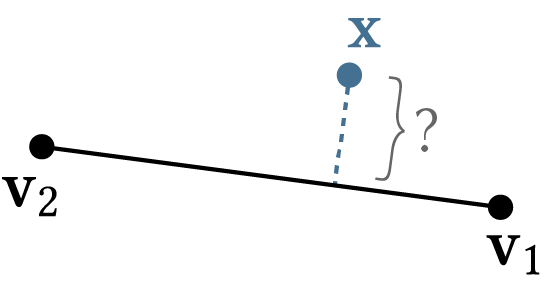
\includegraphics[width=0.8\linewidth]{images/SegmentDistance.png}
   \caption{In this picture, our $p_{closest}$ is the point $p(t) = v_1 + ts$, where $t=\frac{(\mathbf{x}-\mathbf{v}_{1})\cdot (\mathbf{v}_{2}-\mathbf{v}_{1})}{(\mathbf{v}_{2}-\mathbf{v}_{1})\cdot (\mathbf{v}_{2}-\mathbf{v}_{1})}$.}  
\end{marginfigure}

\subsection{Qaudratic Error Curve Simplification}



\chapter{Esoterica!}

The fun chapter composed entirely of everyone's obscure resources!

\section*{Nick Sharp}
https://web.evanchen.cc/handouts/bary/bary-full.pdf
(IMO, IOI, Putnam, ACM ICPC, Codeforces, etc)
https://cses.fi/book/book.pdf

\section*{Justin Solomon}
Troutman and Gelfand/Fomin variatonal calculus
https://web.stanford.edu/~boyd/cvxbook/bv\_cvxbook.pdf
https://www.matrixcalculus.org/
https://www.matrixcalculus.org/matrixcalculus.pdf
https://www.matrixcalculus.org/tensorcalculus.pdf

\section*{Anthony Hong}
https://tikzcd.yichuanshen.de/
https://tikzit.github.io/
https://www.jmilne.org/not/CDGuide.html


\footnotesize
\twocolumn
\bibliographystyle{acm}
\bibliography{biblio1}
\onecolumn

\end{document}
